\chapter{卷积神经网络}
\label{chap:convolutional-networks}

先做一个思想实验：训练好一个能识别竖直边缘的全连接网络。它在图像左上角学会了“相邻像素左亮右暗”这一模式，靠的是连接到左上角那几个特定像素的权重。现在把同一条边缘平移到右下角——在把图像展平成一维向量后，右下角对应完全不同的几个坐标，也就是完全不同的一组权重，而这些权重并没有在左上角的样本中学过。于是网络很可能认不出右下角的这条边缘。要让它在每个位置都能识别，理论上必须让每种边缘在每个位置都出现足够多的训练样本，这显然代价高昂。

这个困难暴露了全连接结构处理图像的两个失配。其一，它把空间上相邻的像素和相距很远的像素同等对待，但判断“边缘”“拐角”这类局部模式，真正有用的信息几乎都来自邻近像素。其二，它让每个位置使用各自独立的权重，于是“在一处学会的规则”无法在结构上自动搬到另一处。然而图像数据恰好有两个鲜明特点：有意义的模式由邻近像素构成，而且同一种模式（一条边缘、一个色块）可能出现在画面任何位置。这就提出了本章的核心问题：\emph{怎样让网络保留空间结构，并让同一种识别规则在多个位置复用}？第~\ref{chap:feedforward-networks}章建立的多层非线性表示提供了基础，卷积神经网络则通过改变连接范围和权重复用方式来回答它。

卷积神经网络用同一组共享权重处理各个局部窗口，再由非线性激活和逐层组合，把局部的边缘、纹理逐级拼成部件乃至物体的预测。由于同一权重在前向计算中被反复使用，学习时就必须把所有位置传回的梯度汇集到这一个权重上；增加深度又改变了信息和梯度经过的路径，带来新的训练问题。本章的推进路线是：先精确定义卷积这一局部运算及其各种边界和采样约定（\ref{sec:cnn-convolution}节），再说明卷积层、池化层、归一化层如何组织成完整网络及经典架构（\ref{sec:cnn-structure}节），然后解决共享权重下的参数初始化与反向传播（\ref{sec:cnn-learning}节），接着介绍支持超深网络的跨层连接（\ref{sec:cnn-extensions}节），最后从理论上分析这种结构能表达什么、能否优化、泛化风险如何（\ref{sec:cnn-theory}节），并落到图像分割与生成等需要保留位置的任务上。激活函数、损失和链式法则沿用前章；结构约束与样本风险之间的统计联系可参考\BookChapterRef{chap:deep-learning-theory}{卷3《基础、理论与可信性》第8章“深度学习的可学习性”}。

\section{卷积神经网络概述}
\label{sec:cnn-overview}

先用一个具体数字看清全连接处理图像为何不可行。设一张彩色图像有$224\times224$个像素，每个像素包含红、绿、蓝三个颜色数值，展平后的输入维度为$224\times224\times3=150528$。若把它连接到$1024$个隐藏单元，仅这一层的权重就有$150528\times1024=154140672$个——还没有算偏置和后续各层。这个数字揭示了两个问题：一是参数量随输入像素数线性膨胀，极易过拟合并消耗巨大存储；二是这种稠密连接把每个输入坐标与每个隐藏单元相连，相邻像素和远隔像素被同等对待，每个位置还可以学到互不相干的局部规则，空间结构信息在展平的瞬间就丢失了。卷积要改变的，正是连接范围和权重复用这两件事。

针对图像的两个特点，可以分别施加两种结构约束。\term{局部感受野}（local receptive field）针对“模式由邻近像素构成”：让一个输出单元只读取输入中的一个小邻域（如$3\times3$窗口），把一次计算限定在附近的若干位置，而不与整张图相连。\term{参数共享}（parameter sharing）针对“同一模式出现在多处”：让图像上不同位置的输出单元使用\emph{同一组}权重，相当于把同一种局部识别规则（比如“检测竖直边缘”）像一把滑动的尺子一样重复应用到整张图像。二者回答不同的问题：局部连接决定一次计算\emph{读取哪里}，参数共享决定不同位置\emph{是否使用同一规则}；需要注意，只限制读取范围并不会自动带来共享——若不共享，各位置仍各自拥有一套权重。

\term{卷积神经网络}（convolutional neural network, CNN）就是把这种\emph{共享的局部计算}与非线性变换逐层堆叠起来，从数据中端到端地学习局部特征及其组合。这里需要引入“通道”这一组织方式。输入图像通常不止一个数值平面：彩色图像的红、绿、蓝就是三个\term{通道}（channel），每个通道是一张与图像等大的数值平面。在网络内部，每个空间位置会并列保存若干种不同的局部特征（如一个通道专门响应某种边缘），同一种特征在所有位置的响应合起来称为一张\term{特征图}（feature map）；一个输出通道就是“一种局部响应在所有输出位置上组成的数值平面”。因此普通密集卷积中，每种输出响应使用一组覆盖全部输入通道的权重，$64$个输出通道意味着$64$组不同的权重（对应$64$种被检测的局部模式），而不是$64$个空间位置。

参数共享带来的节省可以直接核算。对三个输入通道、$64$个输出通道的$3\times3$卷积层，每组权重在三个输入平面上各覆盖一个$3\times3$窗口，权重总数为$3\times3\times3\times64=1728$，再加每个输出通道一个偏置，共$64$个。这个数量只由核尺寸和通道数决定，与图像多大无关：图像变大后，同一组核只是在更多位置滑动，参数数保持不变。对比前面全连接层的一亿多个权重，差异来自两个方面——每个输出只看一个$3\times3$邻域（而非全部像素），且所有位置共用权重（而非各学一套）。需要说明，参数量少并不自动等于表达能力弱：全连接层输出一个隐藏向量，卷积层输出多张保留空间位置的特征图，二者的能力还取决于各自保留了什么信息以及后续如何组合。

共享局部规则还带来一种与“物体移动”有关的重要性质，初学时常与另一个概念混淆，这里先区分清楚。\term{平移等变性}（translation equivariance）指\emph{特征响应对位置保持同步}：输入中的图案移到哪里，输出特征图中的对应响应就移到哪里，相当于“检测结果跟着物体走”。\term{平移不变性}（translation invariance）则指\emph{最终输出不随平移改变}：物体移动后，网络给出的类别仍然相同。二者的差别在不同任务中至关重要：图像分类通常希望物体平移后类别不变（需要不变性），而图像分割必须让输出的轮廓随物体一起移动（需要等变性、不能丢弃位置）。步长为一的卷积在无限网格上天然与平移可交换（即具有等变性）；但在有限图像上，边界处理、下采样和最终的汇聚读出都会改变这一性质。要从“随位置移动的特征”得到“与位置无关的类别”，还需要池化等汇聚操作，具体条件见后文池化部分。

最后说明卷积的适用范围。这套结构假设数据具有三个性质：排列在\emph{规则网格}上、邻近位置\emph{局部相关}、同一种模式在不同位置\emph{重复出现}。图像是二维网格，音频波形和时间序列是一维网格，医学体数据是三维网格，都符合这些假设；序列任务还须限制只读取已发生的位置，避免“看到未来”。但如果输入的各个坐标只是含义不同的表格字段（年龄、收入、邮编……），交换相邻字段通常会改变含义，同一种局部规则也无法沿字段排列重复使用，这时卷积就不适用。是否采用卷积，取决于数据结构是否真的与这些假设相符。

局部处理与逐层汇聚的思想早于今天的大规模深度学习。Fukushima于1980年提出的Neocognitron交替组织局部模式检测与汇聚，使高层能够组合低层响应，并容忍一定的位置变化。它借鉴视觉系统的分层处理，但采用的学习机制与今天端到端反向传播的CNN不同；第~\ref{sec:neural-biological-system}节已介绍这条视觉启发线索\scite{fukushima1980}
到20世纪90年代，LeCun等将可学习卷积、降采样和梯度学习结合，用于手写字符和文档识别。1998年的LeNet-5展示了从像素到类别联合学习的完整系统：任务损失同时决定局部特征与后续分类。多层结构已进入实际识别系统，大规模视觉训练所需的数据和计算条件仍在发展\scite{lecun1998}

卷积结构解决了连接组织问题，深层网络能否有效训练仍是另一道关口。2006年，Hinton、Osindero和Teh提出深度信念网络的逐层学习方法：先学习一层隐表示，再把该表示作为下一层的训练数据，并对整个生成模型作后续微调。\term{逐层预训练}就是先分别为各层寻找有用的初始表示，减少从随机参数同时训练全部层的困难。这项工作为研究深层表示提供了可操作的训练途径，是理解随后深度学习兴起的一项重要进展。它研究的是生成式深层模型，原文的微调采用对比形式的wake--sleep算法，与后来判别式CNN的直接监督训练具有不同的目标和步骤\scite{hinton2006deepbelief}

\Needspace{14\baselineskip}
另一条路线继续探索直接用监督信号训练卷积网络。GPU能够并行执行大量规则乘加，使更宽、更深的模型获得实际可用的训练速度。Cireșan等在2011年报告了GPU上的可配置卷积网络，并在多个图像识别数据集上研究直接反向传播训练。这项工作把卷积训练的规则乘加交给GPU执行，为随后扩大模型和数据规模积累了实现经验\scite{ciresan2011cnn}
有标签数据集的扩大提供了更多视觉变化，GPU实现则让这些样本能够用于更大模型的迭代训练。结构、学习方法、数据与计算因而共同决定了当时可以实际训练的系统。

2012年，AlexNet在ImageNet大规模图像分类中将五个卷积层、ReLU、GPU训练、数据增强和全连接层中的Dropout组合起来，以监督学习从像素学习类别判别。论文报告的ILSVRC-2012参赛系统取得$15.3\%$的top-5测试错误率，第二名为$26.2\%$；这里的top-5错误指正确类别未进入前五个预测。$15.3\%$对应多个网络的组合，并包含额外ImageNet数据预训练；它衡量的是这套参赛系统，单个网络的误差另有报告。这个结果清楚展示了大规模学习特征相对于当时参赛方案的优势，推动卷积网络成为视觉研究的重要路线。这里的预训练是在更大标签集上的监督训练，与2006年的逐层生成式预训练不同\scite{krizhevsky2012}

此后的架构发展把问题进一步拆开：VGG用连续小核组织深度，GoogLeNet用多分支与通道压缩分配计算，Highway和ResNet为跨层信息提供路径，DenseNet让后层直接复用旧特征。它们将在本章相应小节中展开。把这段历史连起来，CNN的发展既包含“如何利用空间结构”的持续改进，也包含“如何让深层表示学得出来”的训练进展；深度学习的兴起是这些进展与数据、计算条件共同作用的结果。

\section{卷积运算}
\label{sec:cnn-convolution}

本节先把“卷积”这一步局部计算精确定义清楚。理解它的关键是抓住四个可以独立调节的“旋钮”：\textbf{核}决定每个局部窗口内各位置以多大权重组合；\textbf{边界规则}决定窗口滑出图像范围时读取什么；\textbf{步幅}决定相邻两个窗口相隔多远；\textbf{空洞率}决定窗口内部是密集采样还是跳过一些位置。此外还有一个看似奇怪、实则在图像生成中很常用的“反向”运算——转置卷积。本节逐一固定这些约定，再推广到多通道和不同实现。读者需要特别注意：深度学习里说的“卷积”通常省略了数学卷积中的核翻转，实际用的是互相关；这一区别下面会用算例讲清。数学卷积按固定核线性组合输入，并在相应边界下与平移交换（参考\BookSectionRef{sec:signal-analysis-lti-convolution}{卷1《数学准备：计算、分析与几何》第8章“信号”第8.3.3.1节“线性时不变条件下的卷积映射”}）。

\subsection{从数学卷积到网络运算}
\label{sec:cnn-convolution-definition}

卷积这个词来自信号处理，其核心直觉是“\emph{用一个小的权重模板（核）在输入上滑动，每到一处就计算模板与该处局部内容的匹配程度}”。数学卷积用\emph{相对位置}决定权重：对有限支撑的一维核$k$，离散输出为
\[
  y_i=\sum_a k_a x_{i-a}.
\]
本章的输入与核都是有限数组；输入在原矩阵以外如何取值要另行约定（补零或周期延拓），再通过裁剪决定保留哪些输出位置。

这里有一个初学者最容易困惑的细节：核的方向。二维核的数学卷积要同时反转行、列方向，相当于把核旋转$180$度后再滑动；而网络实现通常\emph{省去这次旋转}，直接按存储的核方向去匹配窗口，这种运算称为互相关。为什么要做这个区分？因为对一个需要学习的核来说，翻转与否只是把参数换了个排列位置，网络能学到的函数集合完全相同；但对一个预先给定、带特定方向含义的核，翻不翻转会改变结果。第~\ref{sec:cnn-matrix-operation}节会用同一个窗口并排比较这两种运算，让符号差异落到具体数值上。

固定核、完整网格及一致的边界约定下，输入平移会使输出同步平移。在线性系统分析中，这项性质称为平移不变性；描述网络的输入输出对应关系时，通常称为平移等变性。二者在此对应同一等式$L(T_rx)=T_r(Lx)$，含义都是输出随输入一起移动，只是两个领域的用语习惯不同。这一等式的成立是有条件的：有限图像上的边界、裁剪和跨步都会限制可用的平移范围；CNN还会学习核权重并在层间插入非线性，整个网络的输入输出关系因此超出了单纯的线性卷积。卷积核也可以含正、负权重，其尺度由学习目标和参数约束决定，不能把它理解成只能做平均的平滑模板。

\subsection{实际应用中的卷积}
\label{sec:cnn-practical-convolution}

\subsubsection{矩阵卷积：翻转与局部求和}
\label{sec:cnn-matrix-operation}

二维数据把单个位置扩展为行、列两个索引。本节采用从零开始的空间索引，输入矩阵为$\bm X\in\mathbb R^{h\times w}$，核为$\bm K\in\mathbb R^{k_h\times k_w}$，元素分别记为$x_{i,j}$和$k_{a,b}$。核索引$a,b$也从零开始。完整二维数学卷积写为
\begin{equation}
  y_{i,j}=\sum_{a=0}^{k_h-1}\sum_{b=0}^{k_w-1}
    k_{a,b}x_{i-a,j-b}\text{。}
  \label{eq:cnn-matrix-convolution}
\end{equation}
输入在原矩阵以外如何取值，需要另行约定。若只保留核完全落在输入内的位置，将输出重排成从零开始的索引，相当于先把核旋转$180$度，再在输入上滑动，对每个窗口作逐元素乘积和求和。

这里的重排需要区分原卷积坐标与窗口坐标。设$h\geq k_h$、$w\geq k_w$，原式中核完整落在输入内的输出坐标$(u,v)$满足$k_h-1\leq u\leq h-1$、$k_w-1\leq v\leq w-1$，因为最小的读取坐标分别为$u-(k_h-1)$和$v-(k_w-1)$。若改用窗口左上角$(i,j)$作为新坐标，原输出坐标就是$(i+k_h-1,j+k_w-1)$。将重新编号的输出记为$\bar y_{i,j}$，并在求和中换用$a'=k_h-1-a$、$b'=k_w-1-b$，便有
\[
  \begin{aligned}
    \bar y_{i,j}
      &=y_{i+k_h-1,j+k_w-1}\\
      &=\sum_{a'=0}^{k_h-1}\sum_{b'=0}^{k_w-1}
         k_{k_h-1-a',\,k_w-1-b'}x_{i+a',j+b'}\text{。}
  \end{aligned}
\]
此时$i=0,\ldots,h-k_h$、$j=0,\ldots,w-k_w$。输入索引随$a',b'$增大而向右下移动，核索引则沿两轴反向，这正是旋转核后再按窗口求和的来源。

用以下教学矩阵固定输入与权重：
\begin{equation}
  \bm X=\begin{bmatrix}
    1&2&3&4\\5&6&7&8\\9&10&11&12\\13&14&15&16
  \end{bmatrix},\qquad
  \bm K=\begin{bmatrix}1&0\\0&-1\end{bmatrix}\text{。}
  \label{eq:cnn-matrix-example}
\end{equation}
图~\ref{fig:cnn-kernel-flip}把同一窗口的两种运算并排比较。旋转后的核为$\left[\begin{smallmatrix}-1&0\\0&1\end{smallmatrix}\right]$，左上窗口给出$-1+6=5$。步长为一且不填充时，核有$3\times3$个合法位置，这里的每个数学卷积输出都是$5$。


本例$k_h=k_w=2$，所以重新编号后的左上输出$\bar y_{0,0}$对应原数学卷积的$y_{1,1}$。原式的$(0,0)$不属于核完整落在输入内的输出坐标；两种编号不能直接当成同一位置。

\begin{figure*}[htb]
  \centering
  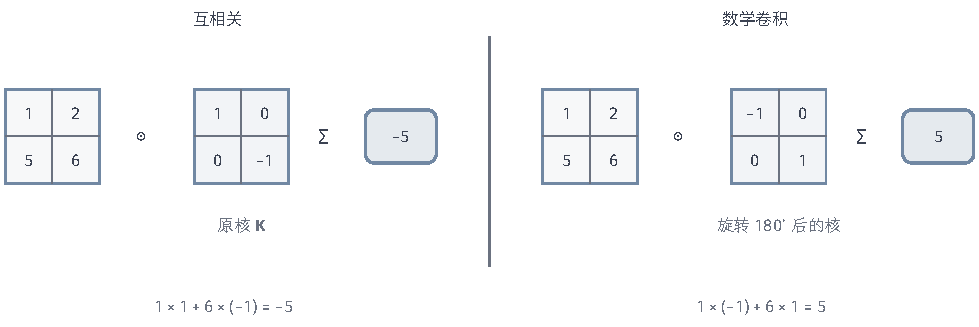
\includegraphics[width=165.767mm]{figures/05-neural-network-models/00-shared/tikz/cnn-kernel-flip/figure.pdf}
  \caption{核的方向改变输出。输入窗口固定为$\left[\begin{smallmatrix}1&2\\5&6\end{smallmatrix}\right]$，核固定为$\left[\begin{smallmatrix}1&0\\0&-1\end{smallmatrix}\right]$。左侧直接逐元素相乘后求和，得到互相关输出$-5$；右侧先把核旋转$180$度，再求和，得到数学卷积输出$5$。$\odot$表示逐元素乘法，$\sum$表示把四个乘积相加。}
  \label{fig:cnn-kernel-flip}
\end{figure*}
\subsubsection{互相关：保留核的方向}
\label{sec:cnn-correlation-operation}

网络通常省去这次旋转，直接用存储的核权重对窗口求和。这种\term{互相关}（cross-correlation）是按核原有方向匹配局部输入；本章针对实数数据写为
\begin{equation}
  y_{i,j}=\sum_{a=0}^{k_h-1}\sum_{b=0}^{k_w-1}
    k_{a,b}x_{i+a,j+b}\text{。}
  \label{eq:cnn-cross-correlation}
\end{equation}
于是左上窗口得到$1-6=-5$，全部输出构成$3\times3$的常数矩阵，见图~\ref{fig:cnn-sliding-window}。对无方向约束的可学习核，翻转只是参数位置的重新排列，卷积与互相关对应同一类候选映射；对预先给定的核，方向仍会改变结果。深度学习文献和软件通常把这种互相关也称为卷积。下文的网络公式遵循这一惯例，保留“数学卷积”来指明需要翻转的运算。

\begin{figure*}[htb]
  \centering
  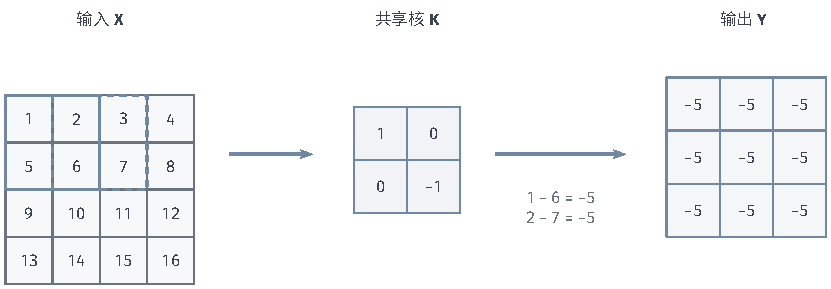
\includegraphics[width=140.723mm]{figures/05-neural-network-models/00-shared/tikz/cnn-sliding-window/figure.pdf}
  \caption{共享核在二维矩阵上滑动的教学例子。蓝色实线和虚线分别框出相邻的两个$2\times2$输入窗口，中间矩阵给出保持原方向的核，右侧矩阵给出互相关输出。每个输出计算窗口左上数值减去右下数值，因此均为$-5$；两个位置使用同一组权重。}
  \label{fig:cnn-sliding-window}
\end{figure*}

\subsubsection{数据填充：确定边界假设}
\label{sec:cnn-padding-operation}

如果不做任何处理，卷积会遇到两个边界问题。一是尺寸缩小：核必须完全落在图像内，$3\times3$核在$4\times4$图上只有$3\times3$个合法位置，每卷积一次特征图就变小一圈，深层网络很快缩没了。二是边缘像素被“轻视”：角落的像素只被一个窗口扫到，而内部像素被多个窗口反复读取，边缘信息参与计算的次数明显偏少。\term{数据填充}（padding）在矩阵外人为补充一圈数值，让核也能完整覆盖边缘附近的位置，从而解决这两个问题。补什么值则体现了对“图外是什么”的不同假设：零填充把外部值设为零；复制填充延续最近的边缘值；反射填充按边界镜像取值；循环填充把图像另一侧的数据接过来（适合本身具有周期性的信号）。这些外部值都是人为构造的，直接决定边缘窗口的计算结果，因此填充不是无关紧要的实现细节，而是一种边界假设。

对式\eqref{eq:cnn-matrix-example}只在右侧和下侧各补一列、一行零，输出就有$4\times4$个位置：
\begin{equation}
  \bm Y=\begin{bmatrix}
    -5&-5&-5&4\\-5&-5&-5&8\\-5&-5&-5&12\\13&14&15&16
  \end{bmatrix}\text{。}
  \label{eq:cnn-padding-example}
\end{equation}
最后一列和最后一行改变，是因为核的负权重落到了补零区域。图~\ref{fig:cnn-padding}标出右上和右下两个窗口：相同的核在内部读取真实数值，在边界则读取约定的零。\term{valid填充}表示不添加边界值，\term{same填充}通常表示按输入尺寸和步长选择填充，使输出尺寸达到约定值。步长为一时常取输出与输入等大；偶数核可能需要不对称填充，本例就是这种情况。步长大于一时，有些接口以$\lceil h/s_h\rceil$为目标高度，具体左右分配还需核对所用约定。


\begin{figure*}[htb]
  \centering
  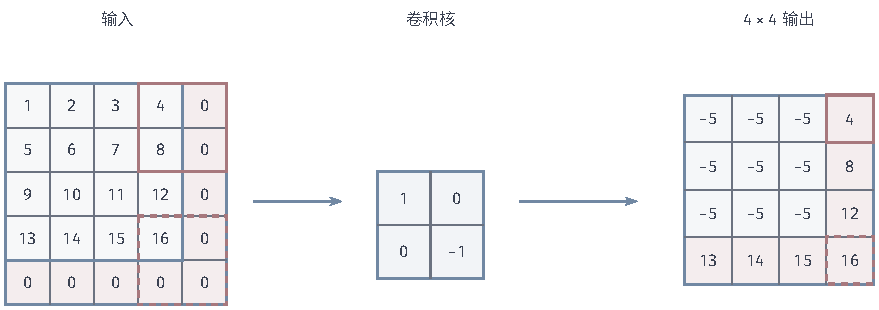
\includegraphics[width=148.791mm]{figures/05-neural-network-models/00-shared/tikz/cnn-padding/figure.pdf}
  \caption{不对称零填充与边界输出。蓝色框内是原$4\times4$输入，浅红色区域是右侧、下侧各新增的一列、一行零。红色实线窗口产生右上输出$4$，虚线窗口产生右下输出$16$，输出矩阵中用相同线型标记对应位置。核为$(1,0;0,-1)$，步长一、空洞率一，计算采用互相关。}
  \label{fig:cnn-padding}
\end{figure*}
\subsubsection{跨步卷积：改变窗口移动间隔}
\label{sec:cnn-stride-operation}

前面默认核每次只移动一格，输出与输入大致等大。有时我们希望\emph{在做局部变换的同时缩小特征图}，比如高层只需要粗略的空间布局、或要降低计算量。\term{跨步卷积}（strided convolution）让核每次沿高、宽分别跳过$s_h,s_w$个输入位置再计算下一个输出，从而直接减少输出位置的密度。在原例中，不填充且$s_h=s_w=2$，只保留窗口起点$(0,0),(0,2),(2,0),(2,2)$，得到$2\times2$的输出，数值仍均为$-5$。图~\ref{fig:cnn-stride}显示，跨步改变的是\emph{窗口起点之间的间隔}（减少了起点数量），窗口内部仍然读取相邻的四个元素，并没有改变核本身。它把“局部变换”和“下采样”合并在一步完成。需要留意其代价：若输入在被跳过的位置之间含有较快的空间变化，隔点采样可能把不同的变化混到一起甚至漏掉细节，这正是信号处理中的混叠问题。


\begin{figure*}[htb]
  \centering
  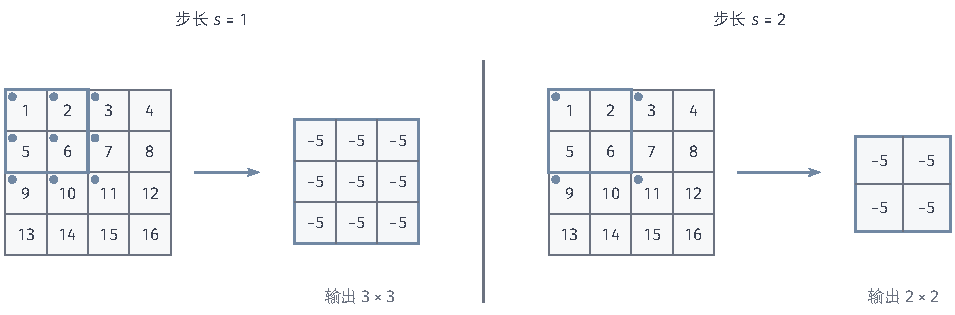
\includegraphics[width=161.766mm]{figures/05-neural-network-models/00-shared/tikz/cnn-stride/figure.pdf}
  \caption{跨步改变输出位置的密度。输入、$2\times2$核和无填充设置保持不变，只将高、宽步长从一改为二。每个蓝色圆点标记一个窗口的左上起点，起点分别形成$3\times3$和$2\times2$的网格；实线框只画出第一个窗口。该教学矩阵的所有窗口都得到$-5$，输出值相同不表示读取的位置相同。}
  \label{fig:cnn-stride}
\end{figure*}
\subsubsection{空洞卷积：改变核内采样间隔}
\label{sec:cnn-dilation-operation}

再考虑另一个需求：希望一个输出能\emph{看到}更大范围的上下文，却又不想增加核的参数量（加大核会带来更多权重和计算）。办法是保持核元素个数不变，但让它们在输入上\emph{隔开}采样。\term{空洞卷积}（dilated convolution）在相邻核元素之间跳过$d_h-1,d_w-1$个输入位置，$d_h,d_w$称为空洞率。原例取$d_h=d_w=2$、步长为一且不填充，左上输出变为$x_{0,0}-x_{2,2}=1-11=-10$，得到$2\times2$的常数输出。此时核仍只有四个权重，但它们覆盖了$3\times3$区域的四个角点而非紧密相邻的四格——\emph{感受野扩大了，参数量和计算量却没有增加}。图~\ref{fig:cnn-dilation}把权重与实际采样位置对应起来；图~\ref{fig:cnn-sampling}再并排区分“核内采样间隔”（空洞）与“窗口移动间隔”（步幅）这两个容易混淆的量。空洞卷积也有代价：重复使用相同空洞率可能在覆盖区域内留下始终读不到的网格位置，所以扩大覆盖范围不等于密集读取了其中所有信息。


\begin{figure*}[htb]
  \centering
  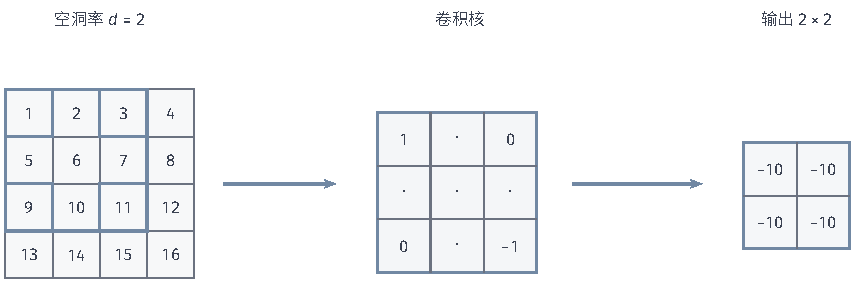
\includegraphics[width=144.766mm]{figures/05-neural-network-models/00-shared/tikz/cnn-dilation/figure.pdf}
  \caption{空洞率二时的实际采样位置。左图彩色小框标出左上输出读取的四格，蓝色外框标出其$3\times3$覆盖区域；中图把原$2\times2$核权重按采样间隔排开，点号表示跳过的位置。数值零占据一个已有核位置，点号处则没有核参数。步长一、无填充时，左上输出为$1-11=-10$，全部输出构成$2\times2$矩阵。}
  \label{fig:cnn-dilation}
\end{figure*}
\subsubsection{统一表达与输出尺寸}
\label{sec:cnn-shape-operation}

把这些设置合在一起，记上下填充为$p_{\mathrm t},p_{\mathrm b}$、左右填充为$p_{\mathrm l},p_{\mathrm r}$，以$\widetilde x_{i,j}$表示在原坐标外扩展的输入值。互相关计算为
\begin{equation}
  y_{i,j}=\sum_{a=0}^{k_h-1}\sum_{b=0}^{k_w-1}
    k_{a,b}\widetilde x_{is_h-p_{\mathrm t}+ad_h,\,
                         js_w-p_{\mathrm l}+bd_w}\text{。}
  \label{eq:cnn-general-correlation}
\end{equation}
有效核尺寸为$e_h=d_h(k_h-1)+1$、$e_w=d_w(k_w-1)+1$，要求填充后的输入至少容纳一个窗口。使用只保留完整窗口的取整规则时，输出尺寸为
\begin{equation}
  \begin{aligned}
    h'&=\left\lfloor\frac{h+p_{\mathrm t}+p_{\mathrm b}-e_h}{s_h}\right\rfloor+1,\\
    w'&=\left\lfloor\frac{w+p_{\mathrm l}+p_{\mathrm r}-e_w}{s_w}\right\rfloor+1\text{。}
  \end{aligned}
  \label{eq:cnn-output-size}
\end{equation}
分子表示窗口起点可以移动的总距离，除以步长后取整得到可移动的次数，再加上起始窗口。这也解释了为什么同样的输出大小可能来自不同的输入大小：不足一个步长的尾部会被舍去。

\begin{figure*}[htb]
  \centering
  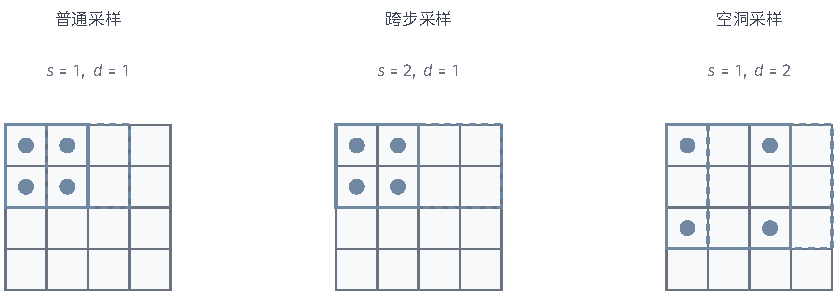
\includegraphics[width=141.792mm]{figures/05-neural-network-models/00-shared/tikz/cnn-sampling/figure.pdf}
  \caption{同一个$2\times2$核的三种采样设置。实线框给出一个输出所覆盖的区域，紫点是该窗口实际读取的位置，虚线框表示下一个水平窗口。普通设置与跨步设置的核内邻距均为一，后者将窗口起点移远；空洞设置将核内邻距增为二，窗口起点仍只移动一格。}
  \label{fig:cnn-sampling}
\end{figure*}

\subsubsection{转置卷积：把局部贡献分配回去}
\label{sec:cnn-transpose-operation}

转置卷积是初学者最容易误解的运算，需要先弄清它\emph{为什么会出现}，再看它做什么。普通卷积把一张较大的特征图压缩成较小的输出（尤其在步幅大于一时）；但在图像分割、生成这类任务中，网络往往需要\emph{反向地把分辨率放大}——从一个粗略的低分辨率特征图，恢复出逐像素的高分辨率输出。如何定义一个与卷积“方向相反”、能把一个输入值扩散到多个输出位置的可学习运算？这就是转置卷积的出发点。

先把普通卷积写成矩阵形式。固定核与输入、输出形状，把输入和输出展平为向量$\bm x$和$\bm y$，忽略偏置，则前向计算是一个线性映射$\bm y=\bm C\bm x$；矩阵$\bm C$的每一行对应一个输出，行中的非零位置标出它读取了哪些输入，共享权重在多行重复出现。\term{转置卷积}（transposed convolution）直接使用这个矩阵的转置：对给定的$\bm v$计算$\bm C^\top\bm v$。从作用上看，普通卷积是“把一个窗口内的多个输入\emph{汇聚}成一个输出”，转置卷积则反过来“把一个输入值按核权重\emph{分配}到多个输出位置”，并把不同输入分配到同一位置的贡献相加。

取原例第一行$(1,2,3,4)$，用一维核$(1,-1)$说明同样的过程。步长为一且不填充时，
\begin{equation}
  \bm C=\begin{bmatrix}
    1&-1&0&0\\0&1&-1&0\\0&0&1&-1
  \end{bmatrix},\qquad
  \bm C^\top\begin{bmatrix}1\\1\\1\end{bmatrix}
    =\begin{bmatrix}1\\0\\0\\-1\end{bmatrix}\text{。}
  \label{eq:cnn-transpose-example}
\end{equation}
图~\ref{fig:cnn-transpose-scatter}逐项展开分配过程。中间两个位置各收到正、负贡献，累加后成为零；转置映射的结果由这些贡献共同确定。这里必须澄清一个常见误解：\emph{转置卷积不是卷积的逆运算，不能把下采样丢掉的信息还原回来}。$\bm C$把四维输入压成三维输出，已经丢失了部分信息；而$\bm C^\top\bm C$一般不等于单位矩阵，所以$\bm C^\top$只是把贡献“铺回去”，铺回的结果由核权重决定，并非恢复原始输入。本例中它执行的是一次重新分配，前向已丢失的信息仍然没有恢复。作为网络中的可学习层时，转置卷积也可以独立学习自己的核参数，与对应前向卷积的核不必相同。


\begin{figure}[htb]
  \centering
  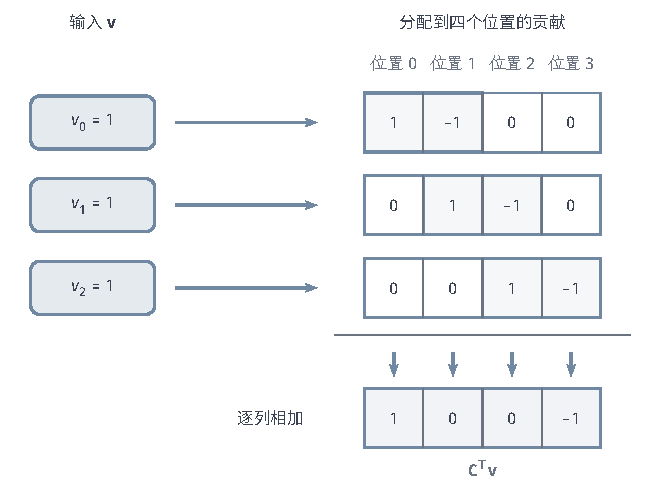
\includegraphics[width=112.000mm]{figures/05-neural-network-models/00-shared/tikz/cnn-transpose-scatter/figure.pdf}
  \caption{转置卷积的分配与累加。输入为$\bm v=(1,1,1)^\top$，核为$(1,-1)$，步长一、无填充。每行分别表示一个输入值对四个输出位置的贡献，紫框圈出两个可能非零的位置；没有贡献的格子记为零。逐列相加得到$(1,0,0,-1)^\top$，中间两格均包含来自不同输入的重叠贡献。}
  \label{fig:cnn-transpose-scatter}
\end{figure}
\FloatBarrier
转置映射的目标长度为何还需要额外选择，可以从普通卷积的取整公式反解。设原输入长度为正整数$n$，对称零填充为非负整数$p$，步长$s$、空洞率$d$和核长$k$均为正整数，有效核长度为$e=d(k-1)+1$。在$n+2p\geq e$、至少容纳一个完整窗口时，普通卷积输出长度为$n'=\lfloor(n+2p-e)/s\rfloor+1$。固定这个正整数$n'$后，向下取整的定义给出
\[
  n'-1\leq\frac{n+2p-e}{s}<n'
  \quad\Longleftrightarrow\quad
  (n'-1)s\leq n+2p-e<n's\text{。}
\]
因此，令$o=n+2p-e-(n'-1)s$，就得到整数余量$0\leq o<s$；它记录最后一个完整窗口之后不足一步的剩余长度。把这一等式解出$n$，并将原输入长度作为转置映射的目标长度，就得到下面的尺寸表达式。反解时仍只接受正的目标长度，并保留上述完整窗口条件。

在一维对称零填充$p$、步长$s$、空洞率$d$和核长$k$的约定下，转置卷积输入长度$n'$对应的输出长度常写为
\begin{equation}
  n_{\mathrm{out}}=(n'-1)s-2p+d(k-1)+1+o,
  \qquad 0\leq o<s\text{。}
  \label{eq:cnn-transposed-size}
\end{equation}
这里$o$是用于选择目标形状的输出填充量：普通卷积取整后，同一个$n'$可能对应$s$种原输入长度。选定目标长度后，前向矩阵的列数及其转置的输出形状才随之确定。$o$是尺寸约定，不表示把$o$个零作为最终输出值附在末尾。二维情形沿高、宽分别使用该式。不对称填充或额外裁剪会改变矩阵的边界行、列，输出形状也要随对应映射确定。跨步转置卷积可理解为先在输入位置之间插零，再进行适当的滤波与裁剪；不同位置的覆盖次数可能不均匀，需要检查输出中的周期性纹理。卷积尺寸与转置关系的系统说明见Dumoulin和Visin的算术指南\scite{dumoulin2016arithmetic}

例如取$k=3$、$d=1$、$s=2$、$p=0$，长度$n=5$与$n=6$都给出$n'=2$：相应计算分别为$\lfloor(5-3)/2\rfloor+1=2$和$\lfloor(6-3)/2\rfloor+1=2$。反解得到$n_{\mathrm{out}}=5+o$，选择$o=0$与$o=1$就分别确定五维和六维目标。两个前向矩阵都有两行，但分别有五列和六列；因此，它们的转置虽然都接收两个数，却输出不同长度的向量。$o$确定的是采用哪一种形状的映射，具体输出值仍由对应矩阵的转置计算。

覆盖不均也可以用一个跨步分配例子直接检查。取三个输入值均为一，核为$(1,1,1)$，步长二、无填充、空洞率一，并取$o=0$，则转置输出长度为七。三个输入分别向位置$\{0,1,2\}$、$\{2,3,4\}$和$\{4,5,6\}$分配贡献，逐位置累加得到$(1,1,2,1,2,1,1)$。中间位置收到的贡献次数交替为一、二，即使输入与核值相同，输出也会出现强弱交替；一般输入和权重还会改变这些贡献的数值。

\subsection{卷积的实现}
\label{sec:cnn-implementation}

固定边界与采样设置，在精确算术下，直接求和、矩阵化和满足适用条件的变换算法可以得到相同的预激活值。矩阵化汇集原有局部点积，Toom--Cook、Winograd与FFT通过变换输入和核来重组乘积，空间可分离路线则利用核的低秩结构（代数算法、数值例子及误差条件参考\BookSectionRef{sec:signal-analysis-fast-transforms}{卷1《数学准备：计算、分析与几何》第8章“信号”第8.4节“卷积映射的快速计算”}）。这里固定本层的批量、通道和采样设置，比较直接计算的成本与变换结果的复用，再说明数据如何存储和读取。

此前的单矩阵例子只保留一个数值平面，现在将第~\ref{sec:cnn-overview}节的多通道组织写成张量。一个通道在全部空间位置上的响应构成一张\term{特征图}（feature map）。单个输入的形状为$\bm X\in\mathbb R^{h\times w\times c_{\mathrm{in}}}$，普通密集卷积的核张量为$\bm W\in\mathbb R^{k_h\times k_w\times c_{\mathrm{in}}\times c_{\mathrm{out}}}$。固定一个输出通道，其核覆盖全部输入通道：对空间窗口和输入通道共同求和，产生一个输出值；换用另一组核权重便产生另一个输出通道。因此输入通道轴参与求和，输出通道轴保留在结果中，图~\ref{fig:cnn-channels}给出了对应示意。

以下比较同一个互相关映射，忽略激活；偏置可在累积完成后加入。设小批量含$n_{\mathrm b}$个输入，输入、输出通道数为$c_{\mathrm{in}},c_{\mathrm{out}}$，输出空间尺寸为$h'\times w'$。记
\[
  q=k_hk_wc_{\mathrm{in}},\qquad m=n_{\mathrm b}h'w'\text{，}
\]
即一个窗口的元素数与全部输出位置数。普通密集卷积需要$c_{\mathrm{out}}qm$次乘加；比较额外存储时，输入、核和最终输出不计入工作区。这里把输入数值与核权重相乘称为\emph{核心乘法}；在变换路线中，相应计数的是变换后输入与核的乘积。固定变换中的加减与常数乘法另外计算。总耗时还包含变换、数据读写与调度，后文据此同时计算新增的工作和存储。

矩阵化把本层的每个窗口作为一列，每个核作为一行。按一致顺序展平后，窗口矩阵为$\bm P\in\mathbb R^{q\times m}$，核矩阵为$\bm W_{\mathrm{loc}}\in\mathbb R^{c_{\mathrm{out}}\times q}$；加入偏置$\bm b\in\mathbb R^{c_{\mathrm{out}}}$后，预激活为
\begin{equation}
 \bm Z_{\mathrm{col}}=\bm W_{\mathrm{loc}}\bm P+\bm b\bm1_m^\top.
 \label{eq:cnn-im2col}
\end{equation}
其中$\bm1_m$是$m$维全一向量。这个矩阵等式把同一组局部点积汇集为\term{通用矩阵乘法}（general matrix multiplication, GEMM）；按普通矩阵乘法逐项求和时，乘加量仍与直接计算相同。

\subsubsection{直接计算：逐项求和}
\label{sec:cnn-direct-implementation}

直接算法在每个输出位置逐项累积窗口中的贡献。将批量索引记为$t$，输入元素为$x_{t,i,j,c}$，$w_{a,b,c,o}$表示核位置$(a,b)$上从输入通道$c$到输出通道$o$的权重。记$u(i,a)=is_h-p_{\mathrm t}+ad_h$、$v(j,b)=js_w-p_{\mathrm l}+bd_w$，即式\eqref{eq:cnn-general-correlation}中的实际读取位置，零填充下的核心步骤如下。
\Needspace{13\baselineskip}
\begin{algorithm}[直接多通道互相关]
  \label{alg:cnn-direct}
  \begin{algorithmic}[1]
    \Require 输入$\bm X$、核$\bm W$、偏置$\bm b$及形状、采样设置
    \Ensure 输出预激活$\bm Z$
    \For{每个合法的$(t,i,j,o)$}
      \State $z_{t,i,j,o}\gets b_o$
      \For{每个核位置$(a,b)$和输入通道$c$}
        \State 读取扩展输入$\widetilde x_{t,u(i,a),v(j,b),c}$
        \State $z_{t,i,j,o}\gets z_{t,i,j,o}+w_{a,b,c,o}\widetilde x_{t,u(i,a),v(j,b),c}$
      \EndFor
    \EndFor
  \end{algorithmic}
\end{algorithm}

算法\ref{alg:cnn-direct}的一次外层迭代只负责一个输出。核位置确定空间偏移，输入通道决定读取哪个数值，输出通道决定使用哪组权重；所有贡献加到同一个累积器中，完成后才写出。相邻输出重新使用核，另一个输出通道则使用另一个核，但二者都从同一输入张量取数。

对式\eqref{eq:cnn-matrix-example}的左上输出，顺序计算的四项是$1\times1$、$2\times0$、$5\times0$和$6\times(-1)$，总和为$-5$。零权重是这个例子的特殊取值，普通密集算法仍按四个位置组织计算；只有专门利用零权重结构，才能省去相应乘法。每个窗口含$q$项，一共有$c_{\mathrm{out}}m$个输出，因此乘加量为
\begin{equation}
  O\!\left(n_{\mathrm b}h'w'c_{\mathrm{in}}c_{\mathrm{out}}k_hk_w\right)\text{。}
  \label{eq:cnn-direct-cost}
\end{equation}
直接算法逐项保留局部求和结构，额外工作区可以只包含若干累积器，但算术量随核面积、通道数与输出位置数相乘。相邻窗口存在重叠时，共用输入可以在较近的存储中复用；这种复用属于第~\ref{sec:cnn-engineering}节的数据调度问题。判断一种计算算法时，应先固定数学运算及其乘加量，再考察它在具体存储层次中的执行方式。

\subsubsection{多通道卷积的变换复用}
\label{sec:cnn-transform-reuse}

本层的多个输出通道读取相同的窗口，同一个核又作用于多个位置。这两种共享关系使输入变换能跨输出通道复用，核变换能跨位置复用。
以步长一、无空洞的$3\times3$核为例，Winograd方案用固定矩阵$\bm B^\top,\bm G,\bm A^\top$分别变换输入、变换核并恢复输出，将一个$4\times4$输入块变为$2\times2$输出。其中输入变换矩阵为四行四列，核变换矩阵为四行三列，输出恢复矩阵为两行四列（变换矩阵及恢复等式参考\BookSectionRef{sec:signal-analysis-fast-winograd}{卷1《数学准备：计算、分析与几何》第8章“信号”第8.4.4节“基于余数分解的卷积计算”}）。
固定一个样本的输入块，对输入通道$c$和输出通道$o$，分别形成核变换$\bm U_{c,o}=\bm G\bm W_{c,o}\bm G^\top$与输入变换$\bm V_c=\bm B^\top\bm X_c\bm B$。其中$\bm W_{c,o}\in\mathbb R^{3\times3}$是核在通道$(c,o)$上的空间切片，$\bm X_c\in\mathbb R^{4\times4}$是该输入块在通道$c$上的空间切片。
通道累积与输出恢复写成
\begin{equation}
 \bm Y_o=\bm A^\top\left(\sum_c\bm U_{c,o}\odot\bm V_c\right)\bm A.
 \label{eq:cnn-winograd-channel-reuse}
\end{equation}
式中的乘积按对应位置逐元素相乘，再对全部输入通道求和。输入变换可供多个输出通道复用，核变换可供多个空间块与批量样本复用。
由于输出变换是线性的，先对通道求和再恢复，与逐通道恢复后相加等价，却只需为每个输出通道执行一次恢复。
若同时处理$n_{\mathrm{tile}}$个输入块，在每个变换位置上还可把核组合排成$c_{\mathrm{out}}\times c_{\mathrm{in}}$矩阵，输入组合排成$c_{\mathrm{in}}\times n_{\mathrm{tile}}$矩阵。
这一$F(2\times2,3\times3)$方案的记号依次表示输出块和核的空间尺寸。其变换结果可以组织为十六组通道矩阵乘法，与GEMM组合使用。

实现时将输出切为不重叠的$2\times2$块，各自读取$4\times4$输入块，再恢复四个空间输出并加偏置。
相邻输出块起点相隔两格，输入块重叠两行或两列；边缘不足一块时需要填充或单独处理。
变换核保存十六个系数，而原核只有九个系数，活动值工作区也会扩大；分块可以限制同时保存的变换值。
更大的输出块通常还会增加变换成本和数值敏感性，步长与空洞率改变后也不能直接沿用这些矩阵。

频域路线有相同的通道共享关系。对适当翻转并补零后的核，每个频率上的输出为$\widehat y_o=\sum_c\widehat x_c\widehat k_{c,o}$，随后对各输出通道反变换，并按本层规则裁剪和选取输出位置。
若补零后的二维网格含$N$个位置，核心频域乘加量为$O(n_{\mathrm b}c_{\mathrm{in}}c_{\mathrm{out}}N)$；输入、核和输出的变换成本分别为
\begin{align*}
 \text{输入变换：}\quad &O(n_{\mathrm b}c_{\mathrm{in}}N\log N),\\
 \text{核变换：}\quad &O(c_{\mathrm{in}}c_{\mathrm{out}}N\log N),\\
 \text{输出变换：}\quad &O(n_{\mathrm b}c_{\mathrm{out}}N\log N).
\end{align*}
这里$N$是二维网格的总位置数，复数乘法也不能按一次实数乘法计价。
输入频谱可供多个输出核复用，核频谱在参数不变时可跨样本复用；训练更新参数后需要重算。
Mathieu等研究了在CNN中利用这些复用关系的FFT实现\scite{mathieu2014fft}

将单个空间核分解为若干秩一核，可把二维滤波组织为若干组一维滤波，再将结果求和（分解与计算成本参考\BookSectionRef{sec:signal-analysis-fast-separable}{卷1《数学准备：计算、分析与几何》第8章“信号”第8.4.5节“基于核分离的卷积计算”}）。保留全部非零秩一项时，在相同边界和采样约定下恢复原来的空间核；计算能否减少，还取决于核的秩、输入尺寸与边界处理成本。截断分解会改变本层输出，需要检查近似误差或重新训练。第~\ref{sec:cnn-layer}节的深度可分离卷积则改变通道连接方式，以逐通道空间滤波和逐点通道混合两步构造新的参数结构。

\subsubsection{工程实现与优化}
\label{sec:cnn-engineering}

计算算法确定需要哪些乘积与求和，执行速度还取决于数据如何送入计算单元。\term{分块}（tiling）把相邻输出位置和若干通道放在一起计算，在较近的存储中复用它们共用的输入与核，减少重复读取。块越大，复用机会越多，但寄存器和局部存储需求也越高，可能限制并行度。

矩阵化卷积需要决定如何提供式\eqref{eq:cnn-im2col}中的窗口矩阵。\term{数据展开}（im2col）把窗口复制为连续的列，再调用GEMM；显式保存整个矩阵需要$qm$个元素，还会产生展开读写。\term{隐式GEMM}（implicit GEMM）则从原张量按需形成当前计算块所需的片段，省去完整展开矩阵，代价是加载时的地址计算与边界判断。CUTLASS给出了这种实现方式\scite{nvidiaCutlassConvolution}

另一种选择是\term{间接卷积}（indirect convolution）：保存指向原输入通道向量的地址，由专用内核沿地址取数，避免复制全部窗口数值。它与隐式GEMM的区别在于显式记录取数位置，也需要承担地址表和间接访存的成本；沿地址取数需要专门的执行内核，普通GEMM接收的则是数值矩阵\scite{dukhan2019indirect}

卷积之后的偏置和逐元素激活还可在写出前完成，这种\term{算子融合}（operator fusion）减少中间结果的读写与调用次数。分块、布局和融合可用于不同算法，但收益取决于层形状、精度、硬件及训练或推理条件。完整算子的时间、工作区与数值误差，反映了乘法节省与新增成本的合计结果。存储层次、并行调度与融合的具体实现留到
\BookVolumeRef{vol:systems}{卷12《系统》}展开。

\FloatBarrier

\section{网络结构}
\label{sec:cnn-structure}

理解了单个卷积运算之后，本节把这些运算组装成能完成任务的完整网络。一次局部求和只能产生一组线性响应，而且只对应一种局部模式；要识别多种特征、引入非线性、逐步扩大视野并最终给出可比较的预测，还需要不同类型的层各司其职。下面依次说明卷积层（用多个核并行提取多种局部特征及其通道变体）、池化层（汇聚并压缩空间）、激活与归一化层（引入非线性并稳定训练）、以及面向不同任务的输出头，最后把它们组合成LeNet到GoogLeNet等经典架构，看清每种设计在解决什么具体问题。

\subsection{卷积层}
\label{sec:cnn-layer}

沿用第~\ref{sec:cnn-implementation}节的输入与核张量形状，加入偏置$\bm b\in\mathbb R^{c_{\mathrm{out}}}$。空间和核索引从零开始，通道索引$c,o$从一开始；$x_{i,j,c}$、$w_{a,b,c,o}$、$b_o$分别是输入、核与偏置的元素。输出预激活值$\bm Z\in\mathbb R^{h'\times w'\times c_{\mathrm{out}}}$为
\begin{equation}
  \begin{aligned}
    z_{i,j,o}=b_o+\sum_{c=1}^{c_{\mathrm{in}}}
      \sum_{a=0}^{k_h-1}\sum_{b=0}^{k_w-1}
      w_{a,b,c,o}\widetilde x_{u(i,a),v(j,b),c},\\
    u(i,a)=is_h-p_{\mathrm t}+ad_h,\qquad
    v(j,b)=js_w-p_{\mathrm l}+bd_w\text{。}
  \end{aligned}
  \label{eq:cnn-layer-forward}
\end{equation}
随后通常逐元素应用激活，得到$h_{i,j,o}=\sigma(z_{i,j,o})$。图~\ref{fig:cnn-channels}把式中的通道求和展开，展示同一组输入怎样形成多个输出通道。

\begin{figure*}[htb]
  \centering
  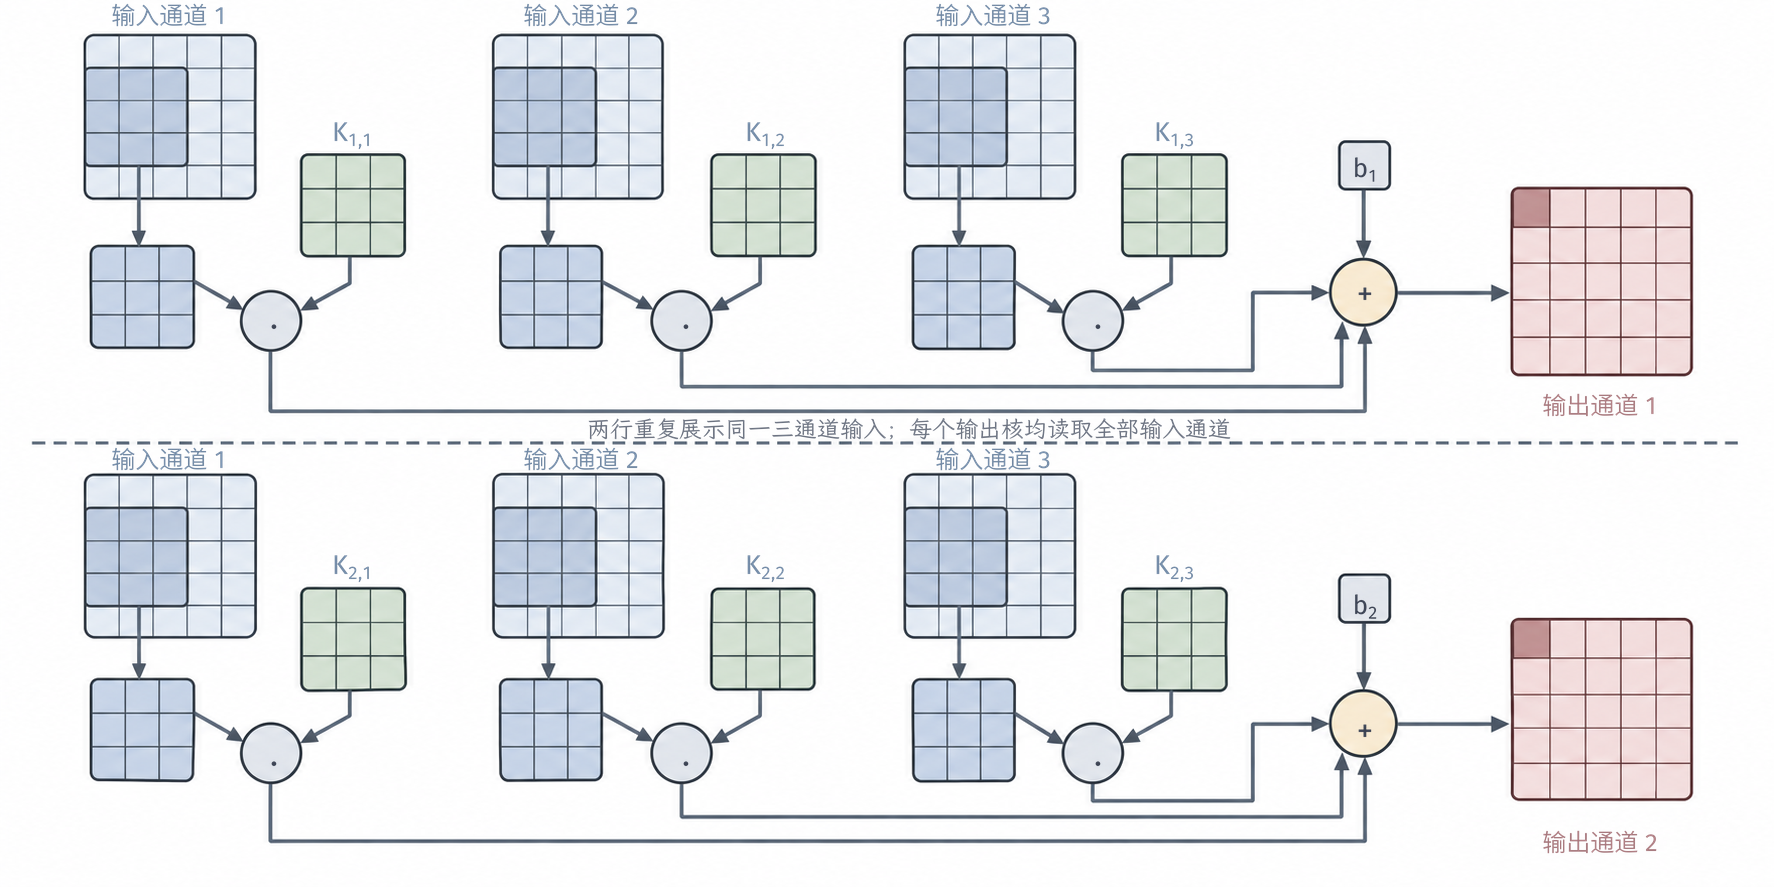
\includegraphics[width=150.199mm]{figures/05-neural-network-models/00-shared/generated/cnn-channels/figure.png}
  \caption{三输入、两输出通道的卷积。每行展示同一输入张量$\bm X$的三个通道；一组输出核包含三个通道切片，各自读取对应输入通道中高亮的局部窗口。各切片完成局部乘加后，三项贡献与偏置一起求和，分别写入右侧输出张量$\bm Z$的两个通道；两个输出平面分别由核1、核2产生。网格只示意通道与局部窗口的关系，不声明实际空间尺寸、步长或填充；核在空间位置间共享，输出尺寸由正文公式确定。}
  \label{fig:cnn-channels}
\end{figure*}

普通卷积层的参数数为
\begin{equation}
  p_{\mathrm{conv}}=k_hk_wc_{\mathrm{in}}c_{\mathrm{out}}
                    +c_{\mathrm{out}}\text{。}
  \label{eq:cnn-layer-parameters}
\end{equation}
空间尺寸没有出现在该式中，却仍出现在式\eqref{eq:cnn-direct-cost}的计算量和活动值存储量中。较大图像可以使用相同参数，但要生成更多响应。因此参数量由核形状决定，计算量和活动值内存还随空间网格扩大。

核为$1\times1$时，每个输出只读取同一空间位置的通道向量。\term{逐点卷积}（pointwise convolution）因此是所有位置共享的通道变换，可以增加、压缩或混合通道，却不直接扩展空间感受野。\term{分组卷积}（grouped convolution）把输入、输出通道分成$g$组，各组只在内部连接；若两类通道数都能被$g$整除，权重数变为$k_hk_wc_{\mathrm{in}}c_{\mathrm{out}}/g$。若每个输入通道单独使用一个空间核，再接逐点卷积混合通道，就得到一种\term{深度可分离卷积}（depthwise separable convolution）：将空间处理与通道混合分成两步。在每个输入通道产生一张中间图的设置下，权重数为$k_hk_wc_{\mathrm{in}}+c_{\mathrm{in}}c_{\mathrm{out}}$，但两步施加的结构约束也与普通卷积不同。

分组卷积的权重数可以按组逐一核算。每组有$c_{\mathrm{in}}/g$个输入通道和$c_{\mathrm{out}}/g$个输出通道，每个组内通道对需要$k_hk_w$个空间权重，因此一组有$k_hk_w(c_{\mathrm{in}}/g)(c_{\mathrm{out}}/g)$个权重。再乘以$g$组，便得到上面的除以$g$的结果。减少的连接也限制了这一层的信息流：某组的输出只能读取同组输入，其他组的信息需要在后续安排跨组混合的操作才能传入。

深度可分离配置则要分别计算两步。逐通道阶段有$c_{\mathrm{in}}$个空间核，每个核含$k_hk_w$个权重，共$k_hk_wc_{\mathrm{in}}$个；它产生$c_{\mathrm{in}}$张中间特征图。逐点阶段的每个输出通道都读取这$c_{\mathrm{in}}$个中间通道，因而需要$c_{\mathrm{in}}c_{\mathrm{out}}$个权重，两项相加就是前述总数。这里每个输入通道产生的中间特征图数为一，即图中所说的深度乘子为一；采用更大的乘子时，中间通道数及两部分权重数都要相应增加。这些权重计数均忽略偏置。

两步分工也说明了结构约束。逐通道阶段先为每个输入通道提取一种空间响应，逐点阶段只在同一位置组合这些响应。若两步之间不加非线性，对固定的输入通道，通往各输出通道的等效空间核只能是该逐通道核的不同倍数；普通卷积则允许每一对输入、输出通道独立设置空间核。因而，参数较少来自对可用空间变换的限制，不能仅凭输入、输出形状相同就把两种层视为等价。

图~\ref{fig:cnn-channel-connectivity-comparison}固定四个输入与四个输出通道，比较通道连接的改变。三个配置采用相同空间核，但读取的通道集合不同；深度可分离配置还通过后续逐点变换建立跨通道交互。

\begin{figure*}[htbp]
  \centering
  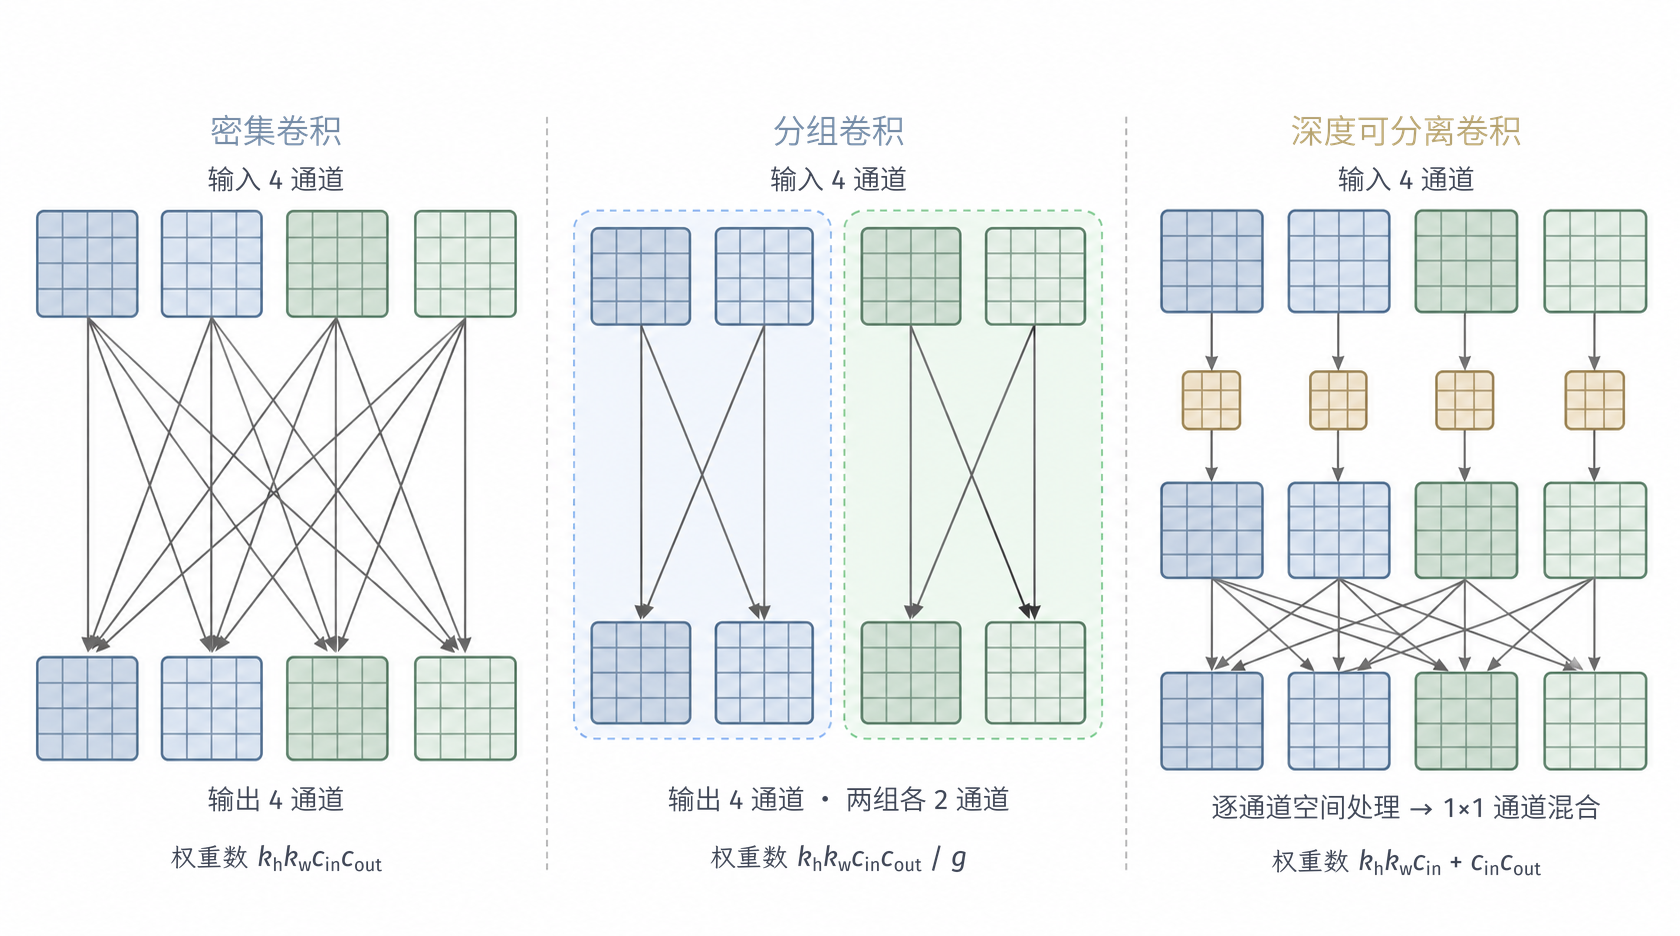
\includegraphics[width=142.240mm]{figures/05-neural-network-models/00-shared/generated/cnn-channel-connectivity-comparison/figure.png}
  \caption{四输入、四输出通道上的三种连接。密集卷积读取所有输入通道；两组卷积仅在各组内部连接；深度可分离卷积先逐通道完成空间处理，再用$1\times1$卷积混合通道。权重数忽略偏置，分组数为二，深度乘子为一。}
  \label{fig:cnn-channel-connectivity-comparison}
\end{figure*}
\FloatBarrier

多层组合让一个高层单元读取更大的输入范围。沿由局部卷积、局部池化和逐点运算组成的单条串联路径，设第$\ell$层的有效核尺寸为$e_\ell$、步长为$s_\ell$，$r_\ell$表示感受野跨度，$j_\ell$表示相邻响应在原输入上的间距。对一个轴，有
\begin{equation}
  r_0=j_0=1,\qquad
  r_\ell=r_{\ell-1}+(e_\ell-1)j_{\ell-1},\qquad
  j_\ell=s_\ell j_{\ell-1}\text{。}
  \label{eq:cnn-receptive-field}
\end{equation}
新增的$e_\ell-1$个间隔，每个在原输入上跨越$j_{\ell-1}$个位置，所以要相乘。以两个空洞率一、步长一的$3\times3$层为例，沿任一轴代入$e_1=e_2=3$和$s_1=s_2=1$，得到
\[
  \begin{aligned}
    r_1&=1+(3-1)\times1=3,& j_1&=1\times1=1,\\
    r_2&=3+(3-1)\times1=5,& j_2&=1\times1=1\text{。}
  \end{aligned}
\]
第二层读取三个相邻的第一层响应，它们各覆盖三个原输入位置，覆盖范围每次只平移一个位置，因此合起来是五个位置，而非九个。高、宽两轴分别计算，便得到$5\times5$；再接同样的一层则为$7\times7$。

若只把第一层的步长改为二，仍有$r_1=3$，但$j_1=2\times1=2$，第二层于是得到$r_2=3+(3-1)\times2=7$、$j_2=1\times2=2$。这里第二层窗口内的相邻响应在原输入上相隔两个位置，故覆盖$7\times7$。一般地，$j_{\ell-1}=\prod_{a=1}^{\ell-1}s_a$是此前各层步长的乘积，空乘积取一；它把当前层的间隔换算回原输入尺度。

这是忽略跨空间统计等非局部操作后的几何感受野；实际梯度和学到的权重可能集中在其中一部分，空洞采样也可能使范围内存在未读取的位置。含归一化的网络还需计入统计量带来的额外依赖，见第~\ref{sec:cnn-activation-normalization}节。填充决定响应中心对应哪个输入位置，边界响应的实际读取范围还会被原图尺寸截断。

\FloatBarrier

\subsection{池化层}
\label{sec:cnn-pooling}

卷积层在每个位置都保留一份局部响应，但后续判断有时并不需要知道某个特征\emph{具体在窗口里的哪个位置出现}，只关心它\emph{是否出现、有多强}。例如判断一张图里有没有眼睛，眼睛在感受野内偏左几个像素往往无关紧要。\term{池化}（pooling）就是对一个小窗口内的数值按某种固定规则汇聚成一个摘要值，通常对每个通道独立进行。它与卷积一样滑动窗口，但有两点本质区别：标准池化\emph{不含可学习权重}（汇聚规则是预先固定的），也\emph{不跨通道混合}。池化一方面逐步缩小空间尺寸、扩大后续单元的相对感受野并降低计算量，另一方面为网络提供了对特征小幅位移的容忍度——这正是从“位置敏感的卷积特征”走向“位置不敏感的类别判断”的关键一环。

设输出位置$(i,j)$在某通道读取的非空有效输入位置集合为$\Omega_{i,j}$，其元素个数为$q_{i,j}$。\term{最大池化}（max pooling）保留窗口内的最大响应，\term{平均池化}（average pooling）保留窗口内的平均响应：
\begin{equation}
  \begin{aligned}
    y_{i,j,c}^{\mathrm{max}}&=\max_{(u,v)\in\Omega_{i,j}}x_{u,v,c},\\
    y_{i,j,c}^{\mathrm{avg}}&=\frac1{q_{i,j}}
                   \sum_{(u,v)\in\Omega_{i,j}}x_{u,v,c}\text{。}
  \end{aligned}
  \label{eq:cnn-local-pooling}
\end{equation}
在式\eqref{eq:cnn-matrix-example}上用不重叠的$2\times2$窗口、步长二且不填充，分别得到
\begin{equation}
  \bm Y^{\mathrm{max}}=\begin{bmatrix}6&8\\14&16\end{bmatrix},\qquad
  \bm Y^{\mathrm{avg}}=\begin{bmatrix}3.5&5.5\\11.5&13.5\end{bmatrix}\text{。}
  \label{eq:cnn-pooling-example}
\end{equation}
最大池化侧重最强响应，平均池化反映整体水平。两者都丢失窗口内的部分信息：仅凭$6$不能知道该窗口的其他三个值，仅凭$3.5$也不能知道四个值的排列。

采用相同窗口与完整窗口取整规则时，池化的输出尺寸可由式\eqref{eq:cnn-output-size}计算。边界规则却要单独核对：最大池化常将无效位置排除，等价于用负无穷填充，而补零会改变全负窗口的最大值；平均池化若把补零位置计入分母，边缘均值会与只除以有效元素数不同。使用向上取整的接口还会保留末尾窗口，并对其边界另作处理；这会给出与本章向下取整约定不同的形状。

\term{全局平均池化}（global average pooling）把每张特征图汇成一个数，得到通道向量$\bm r\in\mathbb R^{c_{\mathrm{in}}}$：
\begin{equation}
  r_c=\frac1{hw}\sum_{i=0}^{h-1}\sum_{j=0}^{w-1}x_{i,j,c}\text{。}
  \label{eq:cnn-global-average-pooling}
\end{equation}
全局最大池化则保留每个通道在全部位置上的最大值。若平移仅对特征图作位置置换，例如循环边界上的整数平移，这两种汇聚都保持结果不变。实际网络中的填充、裁剪和跨步可能改变平移后的特征值和采样位置，此时上述置换条件不再成立。局部池化保留的是窗口中的最大值或平均值，其平移性质也由窗口如何移动决定。

\subsection{激活与归一化}
\label{sec:cnn-activation-normalization}

卷积层本身仍是“加权求和加偏置”的仿射映射，单独堆叠再多也退化为一次仿射，因此卷积之后同样要接非线性激活。ReLU、GELU或SiLU可逐元素作用于特征图，既保留空间和通道形状，又引入非线性。它们的定义、梯度以及与初始化的配合见第~\ref{sec:ffn-activations}节；这里不重复，只强调分工：隐藏层激活决定局部特征如何组合，而末端输出取什么范围（概率还是连续值）由具体任务另行规定。

深层网络在训练中还有一个与激活密切相关的困难：随着前面各层参数不断更新，每一层收到的输入分布都在持续变化，后层不得不反复“追赶”移动的输入尺度；若某些通道的数值变得过大或过小，还容易把Sigmoid、Tanh推入饱和区，拖慢学习。一种直接的想法是，在每一层内部主动把活动值重新拉回到稳定的中心和幅度，再让网络学习如何缩放、平移回去。\term{批归一化}（batch normalization, BN）正是这种做法：它用当前小批量的统计量把特征标准化，再额外学习一个缩放系数和平移量，使网络仍有表达自由度。对卷积特征，均值和方差通常\emph{按通道}、在批量轴和两个空间轴上一起统计；设小批量预激活为$z_{t,i,j,c}$、样本索引$t=1,\ldots,n_{\mathrm b}$，参与统计的元素总数为$m=n_{\mathrm b}h'w'$，则
\begin{equation}
  \begin{aligned}
    \mu_c&=\frac1m\sum_{t,i,j}z_{t,i,j,c},\qquad
    v_c=\frac1m\sum_{t,i,j}(z_{t,i,j,c}-\mu_c)^2,\\
    \widehat z_{t,i,j,c}&=\frac{z_{t,i,j,c}-\mu_c}{\sqrt{v_c+\epsilon}},\qquad
    \bar z_{t,i,j,c}=\gamma_c\widehat z_{t,i,j,c}+\beta_c\text{。}
  \end{aligned}
  \label{eq:cnn-batch-normalization}
\end{equation}
其中$\epsilon>0$防止分母过小。固定通道$c$后，均值与方差汇集全部$n_{\mathrm b}h'w'$个数值，不跨通道求和；同一组可学习参数$\gamma_c,\beta_c$也在这些样本和空间位置之间共享，不为每个像素位置另设一组参数。

全连接前馈网络的BN使用相同原则，但没有空间轴。将一个小批量的特征按行排成$\bm Z_{\mathrm{FFN}}\in\mathbb R^{n_{\mathrm b}\times d}$，固定特征坐标$q$，就只在$\{z_{t,q}:t=1,\ldots,n_{\mathrm b}\}$上统计均值与方差，$\gamma_q,\beta_q$在样本间共享。因此，FFN的“特征级”BN固定一列、跨样本统计，CNN的“通道级”BN固定一个通道、跨样本和空间位置统计。若把卷积特征展平成$n_{\mathrm b}\times(h'w'c_{\mathrm{out}})$后逐列做BN，每个空间位置会分别统计并拥有各自的仿射参数，这与卷积BN不同。其他归一化方法的统计轴对照见图~\ref{fig:training-normalization-axes}。

训练时，共用均值与方差使这些数值的计算相互耦合：一个值改变，可能影响同组其他值的归一化结果。CNN的这种依赖既跨样本，也跨同一通道的空间位置。推理时通常使用训练中累计的均值与方差，使单样本计算固定。累计统计量按实现选定的估计规则更新。常见组合是“卷积—BN—ReLU”，后接BN的卷积层偏置常可省略，因为通道中心化会消除它，BN另有平移参数\scite{ioffe2015batchnorm}

批内独立图像变少时，BN的均值与方差可能更依赖当前批的组成，同一张图像的归一化结果也会随同批其他图像改变。若希望归一化不再读取其他样本，就需要改用单个样本内部的统计量。

当批量较小或批内组成变化较大时，可以改变统计范围。\term{组归一化}（group normalization, GN）把通道分成若干组，对每个样本分别在一组通道及其空间位置上统计均值和方差，然后仍按通道学习缩放与平移。它不需要其他样本提供统计量，训练和推理使用相同的统计范围，但会让同组通道发生统计耦合。组数是结构设置，通道数需要能够均分。GN与BN的区别首先在统计对象：前者独立处理样本，后者使用批内信息。实际训练效果还随任务和批量设置变化\scite{wu2018groupnorm}

这些统计量也改变数据依赖范围。训练态BN通过通道均值与方差连接同批样本的不同空间位置，GN则在训练和推理时都连接同一样本组内的各空间位置；式\eqref{eq:cnn-receptive-field}没有计入这些路径。推理态BN若使用固定的运行统计量，就只是逐点仿射变换，不会额外扩大依赖范围。

归一化、激活和池化的顺序影响计算含义。对平均池化，通常有$\sigma(\operatorname{Avg}(\bm X))\neq\operatorname{Avg}(\sigma(\bm X))$；例如两个响应为$-2$和$1$时，先平均再ReLU得到$0$，先ReLU再平均得到$1/2$。单调逐点激活与不含额外填充值的最大池化可以交换；归一化还读取组内统计量，改变顺序就可能改变输出。各架构因而用明确的模块顺序确定计算；跨架构的训练机制由后续《神经网络的训练》章展开。

\subsection{输出和学习目标}
\label{sec:cnn-output-objectives}

经过若干“卷积—激活—池化”的堆叠，网络得到的还是一张张带空间位置的特征图，而不是最终答案。如何把这些空间特征变成预测，取决于任务要不要保留位置：\emph{整图分类}要把所有空间信息汇聚成一个类别，\emph{逐像素任务}则必须在每个位置给出答案。这一小节给出两种末端的接法；它们复用的是同一套卷积特征，区别只在最后是否丢弃空间轴。

预测整张图像的类别时，需要把空间特征转换为整体得分。可以将末层特征展平后接全连接层，也可以先作全局平均池化再接分类层。设汇聚向量为$\bm r$，类别数为$q$，原始得分为$\bm a=\bm U\bm r+\bm d\in\mathbb R^q$，则多类概率与单样本损失为
\begin{equation}
  p_k=\frac{\exp(a_k)}{\sum_{v=1}^{q}\exp(a_v)},\qquad
  \ell=-\log p_y\text{。}
  \label{eq:cnn-image-classification}
\end{equation}
这里$y\in\{1,\ldots,q\}$为图像标签；训练学习卷积特征与分类层参数，使用时取最大得分类别。回归、二分类和多标签输出可以沿用第~\ref{sec:ffn-output-objectives}节的变换与损失。分类输出的概率由这组类别得分共同归一化，最后一张特征图的数值本身仍是内部响应。

若要预测每个像素的类别，就需要保留或恢复空间轴。设得分张量为$\bm A\in\mathbb R^{h\times w\times q}$，在每个位置单独应用Softmax，可得到$p_{i,j,k}$。给定像素标签$y_{i,j}$，逐位置交叉熵为
\begin{equation}
  \ell_{\mathrm{seg}}=-\frac1{|\Omega|}
    \sum_{(i,j)\in\Omega}\log p_{i,j,y_{i,j}}\text{。}
  \label{eq:cnn-segmentation-loss}
\end{equation}
其中$\Omega$为非空的有标签位置集合，未标注像素不参与求和。每个位置输出多个颜色值或其他连续量时，可改用回归损失。两种输出任务都用卷积特征，却对空间汇聚有不同要求：分类可以舍去具体位置，分割和图像生成必须保留输出与位置之间的对应。

对$n$个独立训练样本，用$\bm\theta$收集所有可学习核、偏置、归一化参数和输出层参数。若网络不含跨样本操作，前向映射可逐样本计算，经验目标可写为
\begin{equation}
  \widehat R_S(\bm\theta)=\frac1n\sum_{t=1}^{n}
    \ell\!\left(\bm f_{\bm\theta}(\bm X_t),\bm Y_t\right)\text{。}
  \label{eq:cnn-training-objective}
\end{equation}
这里$\bm Y_t$统指与任务对应的目标；标量类别标签按式\eqref{eq:cnn-image-classification}处理。像素损失可在单张图像内部先汇聚，再在图像之间取平均。

使用固定统计量的推理态BN符合上述逐样本前向条件，训练态BN则不符合。给定非空批索引集$B$，将整批输入记为$\bm X_B=(\bm X_t)_{t\in B}$，用$\bm F_{\bm\theta}(\bm X_B)_t$表示批预测中对应样本$t$的输出。一次更新所用的数据损失为
\begin{equation}
  L_B(\bm\theta)=\frac1{|B|}\sum_{t\in B}
    \ell\!\left(\bm F_{\bm\theta}(\bm X_B)_t,\bm Y_t\right)\text{。}
  \label{eq:cnn-batch-objective}
\end{equation}
各项损失仍可相加，但每项预测都可能依赖整批输入。求导沿完整批计算图回传，包括均值与方差连接不同样本的路径。分别运行单样本前向会改变归一化统计量及其导数，求导后再平均得到的量一般不同于$\nabla_{\bm\theta}L_B$。若要定义随机分批训练的总体目标，还需给定批抽样规则，再对$L_B$取期望；梯度累积与一次大批前向的区别见第~\ref{sec:training-inexact-gradients}节。正则项、数据增强和优化策略可以加入训练过程，本章重点是结构特有的梯度与信息传递。

\FloatBarrier

\subsection{常见卷积网络架构}
\label{sec:cnn-classic-architectures}

完整架构要在空间精度、特征种类和计算成本之间分配资源。下采样减少空间位置，高层增加通道可以在较粗网格上保存更多特征；末端再根据任务读出。LeNet、AlexNet、VGG和GoogLeNet分别体现了局部到整体、容量扩大、规则小核和多尺度分支的组织方式。图中叠片表示特征张量，正面示意空间网格，叠片示意通道维；深色局部块与算子内部的虚线突出一次局部映射。下方细节用层名对应主链中的算子，独立展示局部计算。全连接层用包含圆形神经元的平面方框表示。蓝色用于卷积特征与全连接，黄色用于池化或降采样，绿色用于少量卷积核细节。主路径从左向右展开，实际尺寸写在各层或阶段下方；绘图尺寸不与张量元素数严格成比例。

\subsubsection{LeNet-5：从局部检测到整体读出}
\label{sec:cnn-lenet}

手写字符的局部笔画需要逐渐组合成整字。LeNet-5交替使用卷积与降采样，先形成小范围响应，再扩大后层能够读取的区域。原网络接收$32\times32$的单通道图像，C1用六个$5\times5$核产生$28\times28\times6$特征；S2降为$14\times14\times6$，C3产生$10\times10\times16$，S4再降为$5\times5\times16$。C5用覆盖整个$5\times5$区域的核得到120个整体特征，接84单元的F6，再计算十类输出，见图~\ref{fig:cnn-lenet}。

F6的84个输出组成表示向量$\bm h\in\mathbb R^{84}$\scite{lecun1998}。原网络为十个类别分别设置同维的参考向量$\bm v_k$，将同一个$\bm h$逐一与它们比较。欧氏径向基函数（Euclidean radial basis function, RBF）读出计算的是平方欧氏距离：
\[
  d_k=\sum_{j=1}^{84}(h_j-v_{k,j})^2
      =\lVert\bm h-\bm v_k\rVert_2^2,
  \qquad k=1,\ldots,10\text{。}
\]
$d_k$越小，表示与第$k$类参考向量越接近；只在这十类中作分类决策时，选择距离最小的类别。原论文按字符的$7\times12$位图设置参考向量，分量为$-1$或$+1$，并至少在初始阶段保持这些向量固定，84维正来自这84个位置。F6需要学习把输入映射到与目标类别参考向量相近的位置。这十个输出是类别不匹配的惩罚值，其大小方向与前节的分类得分相反，也没有直接给出和为一的类别概率。

\begin{figure*}[htb]
  \centering
  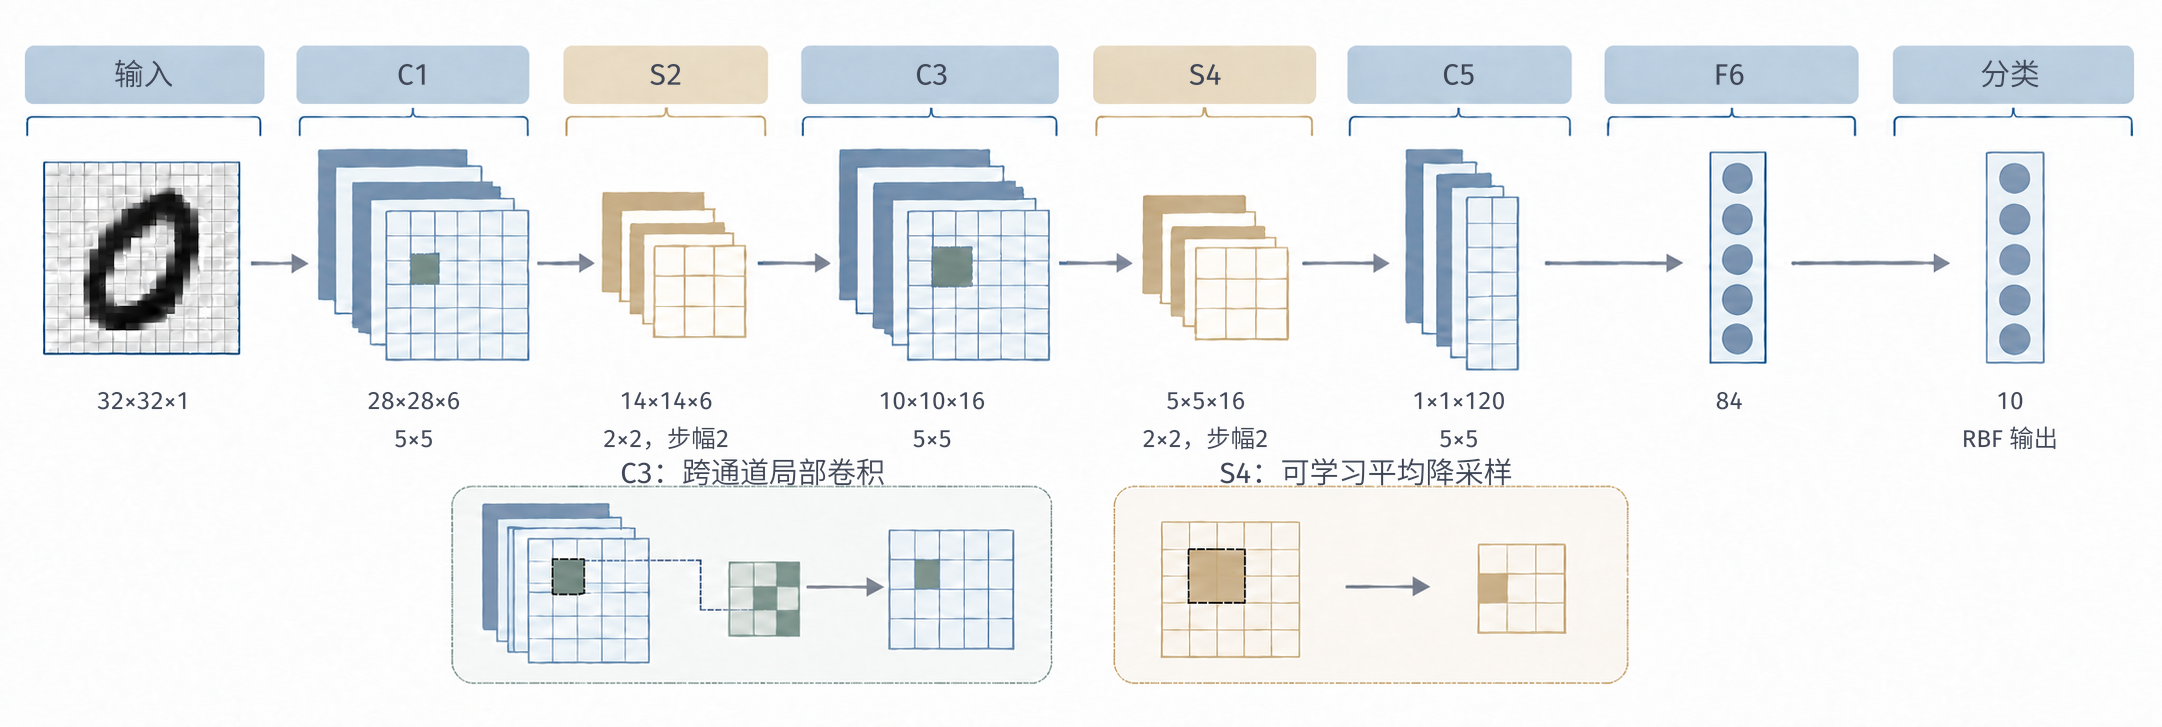
\includegraphics[width=169.000mm]{figures/05-neural-network-models/00-shared/generated/cnn-lenet/figure.png}
  \caption{LeNet-5的层次结构。特征张量用叠片表示，层名与空间、通道尺寸标注在对应图元附近。C1、C3、C5为卷积层，S2、S4为可学习的平均降采样层，F6含84个单元，原始十类读出采用欧氏径向基函数。下方分别展开C3的跨通道局部卷积和S4的平均降采样；网格、叠片数和节点数均为示意，尺寸标签给出真实形状，C3部分通道连接未逐条展开。}
  \label{fig:cnn-lenet}
\end{figure*}

S2和S4采用可学习的降采样：每张特征图的局部求和还经过可学习缩放、偏置和非线性。C3采用指定的部分通道连接，不同输出读取不同的输入组合。C5虽然空间输出为$1\times1$，仍是卷积层；对这里固定的输入形状，它恰好具有整体连接的作用\scite{lecun1998}

教学中常见的“普通卷积—平均池化—ReLU—Softmax”版本使用现代算子重写了这条处理链。它仍按局部检测、空间缩小和整体读出组织计算，但降采样参数、通道连接和输出规则已改变。具体版本由这些计算约定共同确定。

\subsubsection{AlexNet：扩大容量并组织GPU训练}
\label{sec:cnn-alexnet}

自然图像包含更多颜色、纹理和尺度变化，需要更丰富的局部表示。AlexNet包含五个卷积层和三个全连接层；隐藏层使用ReLU，在第一、第二和第五个卷积阶段后作最大池化，在前两个全连接层使用Dropout。卷积主体输出通道依次为$96,256,384,384,256$，前两层分别用较大核快速扩大覆盖范围，后三层用$3\times3$继续组合特征\scite{krizhevsky2012}

图~\ref{fig:cnn-alexnet}采用能明确核算形状的$227\times227$教学输入约定。所有卷积不使用空洞，卷积与池化的空间尺寸均按式\eqref{eq:cnn-output-size}向下取整；三次最大池化均为$3\times3$窗口、步长二、无填充。首层卷积以$11\times11$核、步长四、无填充产生$55\times55$输出，池化降到$27\times27$；第二卷积使用$5\times5$核、步长一、四周各填充二，保持尺度，池化降到$13\times13$；后三层均为$3\times3$核、步长一、四周各填充一，保持该尺度。末次池化形成$6\times6\times256$，展平为9216维，接4096、4096和1000单元。原论文正文写输入$224\times224$，却展示首层55的空间尺寸；在无填充的向下取整规则下二者并不相符。图和本节形状计算统一采用227输入。

\begin{figure*}[htb]
  \centering
  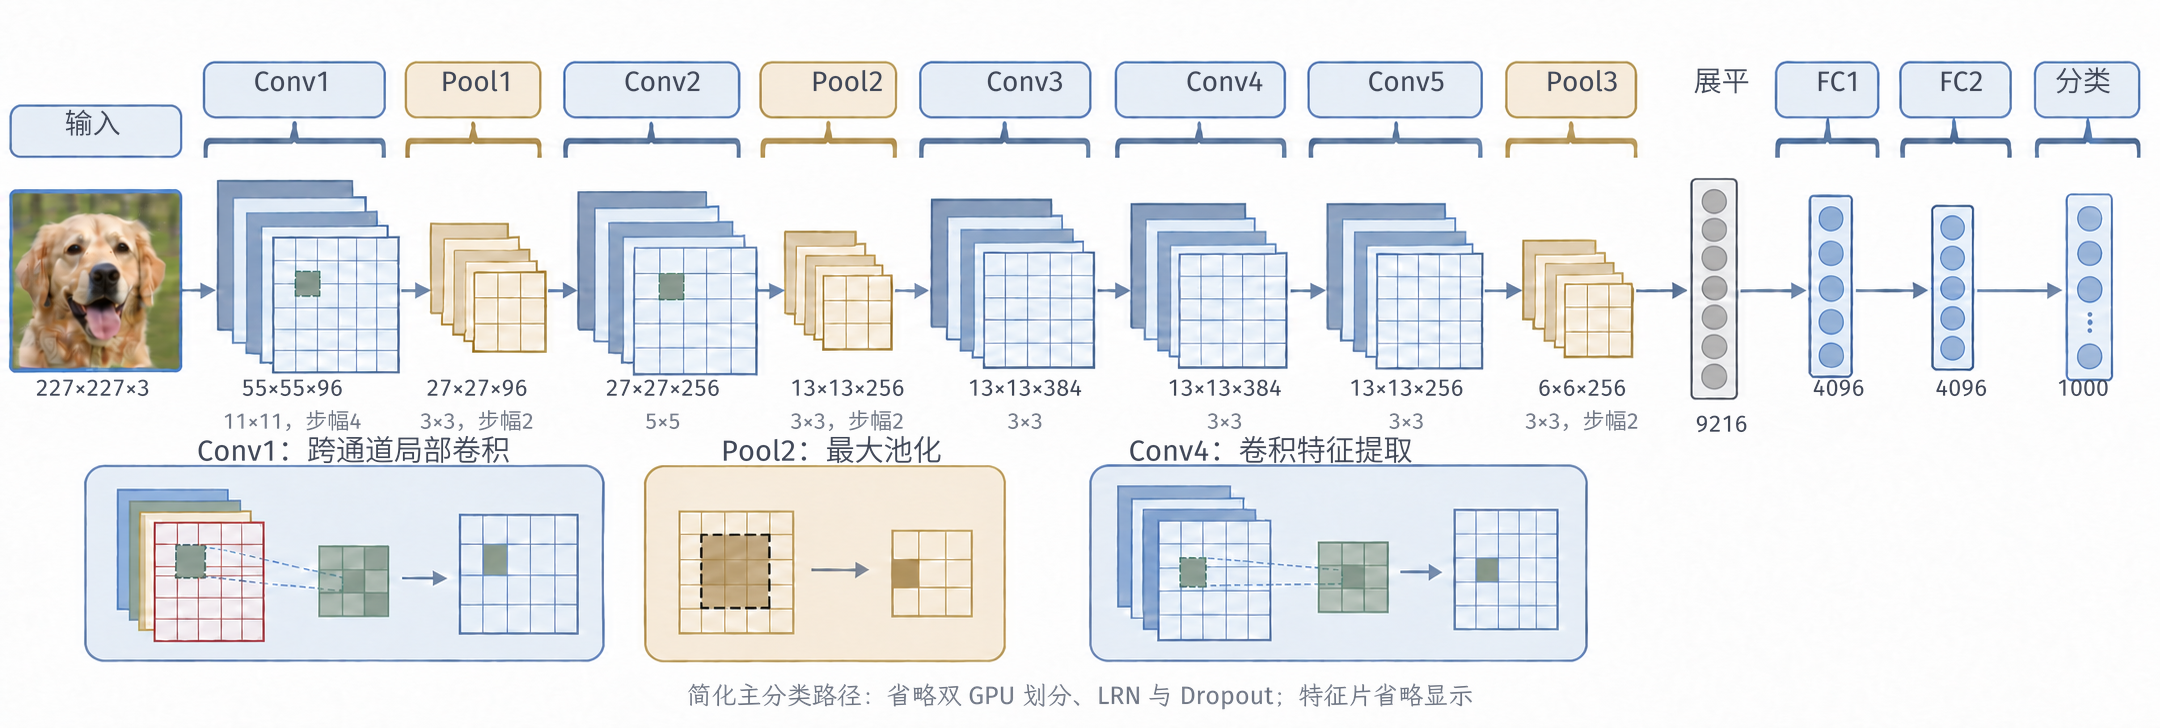
\includegraphics[width=169.000mm]{figures/05-neural-network-models/00-shared/generated/cnn-alexnet/figure.png}
  \caption{AlexNet的五个卷积层与三个全连接层。全部主路径在一行展开，卷积层、最大池化层与全连接层分别绘出；最后一次池化的输出展平为9216维。各层下方给出空间尺寸和通道数，Conv表示卷积，Pool表示池化。下方依次展开Conv1的跨通道卷积、Pool2的最大池化和Conv4的卷积特征提取。网格、叠片和卷积核仅作局部映射示意，各层的实际尺寸与步幅以主链标注为准。此图采用227输入及正文给定的填充约定，省略局部响应归一化、Dropout和原始双GPU的分组细节。}
  \label{fig:cnn-alexnet}
\end{figure*}

容量增加也会把成本集中到尾部。仅9216维到4096维的全连接权重就有$37748736$个，下一层又有$16777216$个；它们与卷积核共享权重的组织不同，是全模型参数量的重要来源。原实现将网络分配到两块GPU，部分层限制跨GPU的通道连接，这也影响了分组方式。ReLU、数据增强和Dropout分别作用于非线性、训练输入变化与正则化；GPU让这些运算可以实际执行，训练设计则规定了参数如何由数据学得。这些条件共同支撑了这套大规模监督系统。

\subsubsection{VGG：以连续小核组织深度}
\label{sec:cnn-vgg}

AlexNet混合不同核尺寸，VGG则研究较规则的小核堆叠。主体使用步长一、填充一的$3\times3$卷积，在阶段末用$2\times2$、步长二的最大池化缩小空间。VGG-16的五个阶段分别含$2,2,3,3,3$个卷积层，通道数为$64,128,256,512,512$；加上三个全连接层，共有16个带权重的层，池化与激活不计入这个数字。VGG-19把后三阶段的卷积数增为四，总计19个带权重层\scite{simonyan2015vgg}

\begin{figure*}[htb]
  \centering
  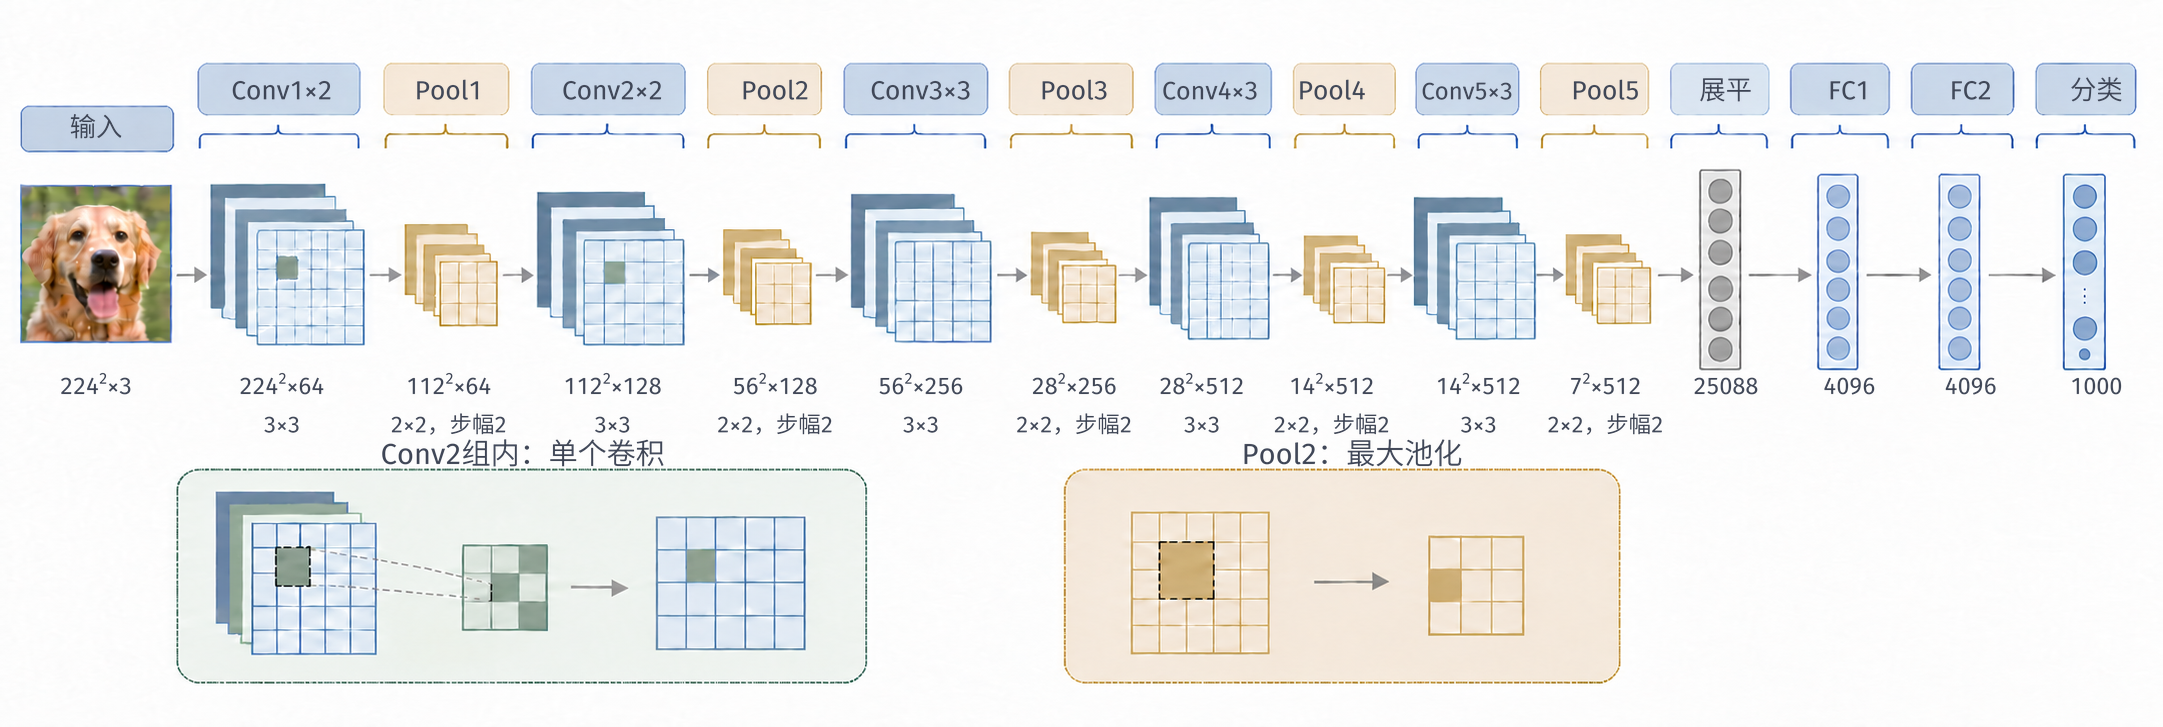
\includegraphics[width=169.000mm]{figures/05-neural-network-models/00-shared/generated/cnn-vgg/figure.png}
  \caption{VGG-16的五阶段卷积主体与全连接尾部。沿用AlexNet的特征叠片、池化、灰色展平及全连接图元；层名和尺寸分别置于对应图元上、下。每个Conv组包含标明次数的$3\times3$卷积并保持空间尺寸，其后的池化单独画出、使空间减半。下方展示Conv2组内单个卷积的代表性局部映射及Pool2的最大池化，并不将单个卷积等同于整个卷积组。13个卷积层加三个全连接层构成16个带权重层。网格、叠片数和节点数仅作示意；$a^2\times c$表示$a\times a\times c$。}
  \label{fig:cnn-vgg}
\end{figure*}

连续小核能够逐层扩大感受野。两个步长一的$3\times3$层覆盖$5\times5$跨度，三个覆盖$7\times7$；若各层通道均为$c$且忽略偏置，两个小核用$18c^2$个权重，单个$5\times5$用$25c^2$个。这个权重比较固定了各层通道数。两个小核之间还加入非线性，候选映射由此改变；相同感受野只描述读取范围。

\begin{figure}[htb]
  \centering
  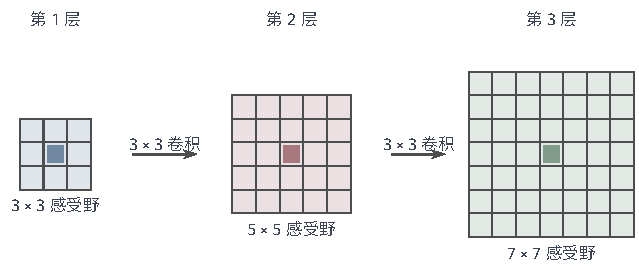
\includegraphics[width=108.158mm]{figures/05-neural-network-models/00-shared/tikz/cnn-receptive-field-stack/figure.pdf}
  \caption{三个步长一、无空洞的$3\times3$卷积逐层扩大几何感受野。彩色方格表示一个高层位置在原输入上可能读取的范围，中心实色格只用于对齐位置；跨度依次为$3,5,7$。图没有计入池化、跨位置归一化或边界填充造成的额外依赖。}
  \label{fig:cnn-receptive-field-stack}
\end{figure}

图~\ref{fig:cnn-receptive-field-stack}还可以沿反向的读取关系理解：第三层的一个位置读取第二层的九个位置，每个第二层位置又读取第一层的九个位置。相邻窗口彼此重叠，最外侧能够涉及原输入的$7\times7$区域。沿途的中间通道和激活决定怎样组合这个区域中的信息。因此，三个小核虽然与一个$7\times7$核具有相同的几何覆盖范围，却通过多次特征变换形成输出；仅凭覆盖范围，不能把两种映射视为等价。

从完整网络看，小核堆叠与阶段间池化承担不同作用。以$224\times224$输入为例，第一阶段的两个卷积始终在$224\times224$网格上组合特征，池化才把网格降到$112\times112$。第二阶段在这个较粗网格上学习128种特征，其后的池化再降到$56\times56$。图~\ref{fig:cnn-vgg}中的每个卷积组都按这个方式展开：组内改变特征内容，组间改变空间精度和后续计算规模。

空间缩小并不意味着卷积运算量按同样比例减少。对步长一的$3\times3$卷积，忽略边界差异，乘加次数约为$9hwc_{\mathrm{in}}c_{\mathrm{out}}$。若高、宽分别减半，同时输入、输出通道都加倍，空间位置数减少到四分之一，通道组合数却增至四倍，乘加次数大致不变；输出活动值数$hwc_{\mathrm{out}}$则减半。VGG各阶段的首层与通道不再增加的后层还要按实际形状单独核算，不能只用网格大小判断成本。

这种规则结构便于分阶段核算形状，但高分辨率阶段仍需保存大量活动值，经典VGG的4096单元全连接尾部也有大量参数。统一的小核安排了深度和读取范围，串联变换中的梯度传播与训练退化仍需通过学习方法和连接设计处理。

\subsubsection{GoogLeNet：在模块内分配多个尺度}
\label{sec:cnn-googlenet}

连续小核把不同尺度安排在不同深度。若希望同一层同时处理不同范围，可以把输入送入并行分支。\term{Inception模块}将同一输入分别交给$1\times1$、$3\times3$、$5\times5$局部处理及池化分支，再沿通道轴拼接。较大核前先用$1\times1$压缩通道，池化分支保持空间尺寸后也可用逐点卷积调节通道。各分支需要相同高、宽，通道数则可以不同，见图~\ref{fig:cnn-inception}。

\begin{figure*}[htb]
  \centering
  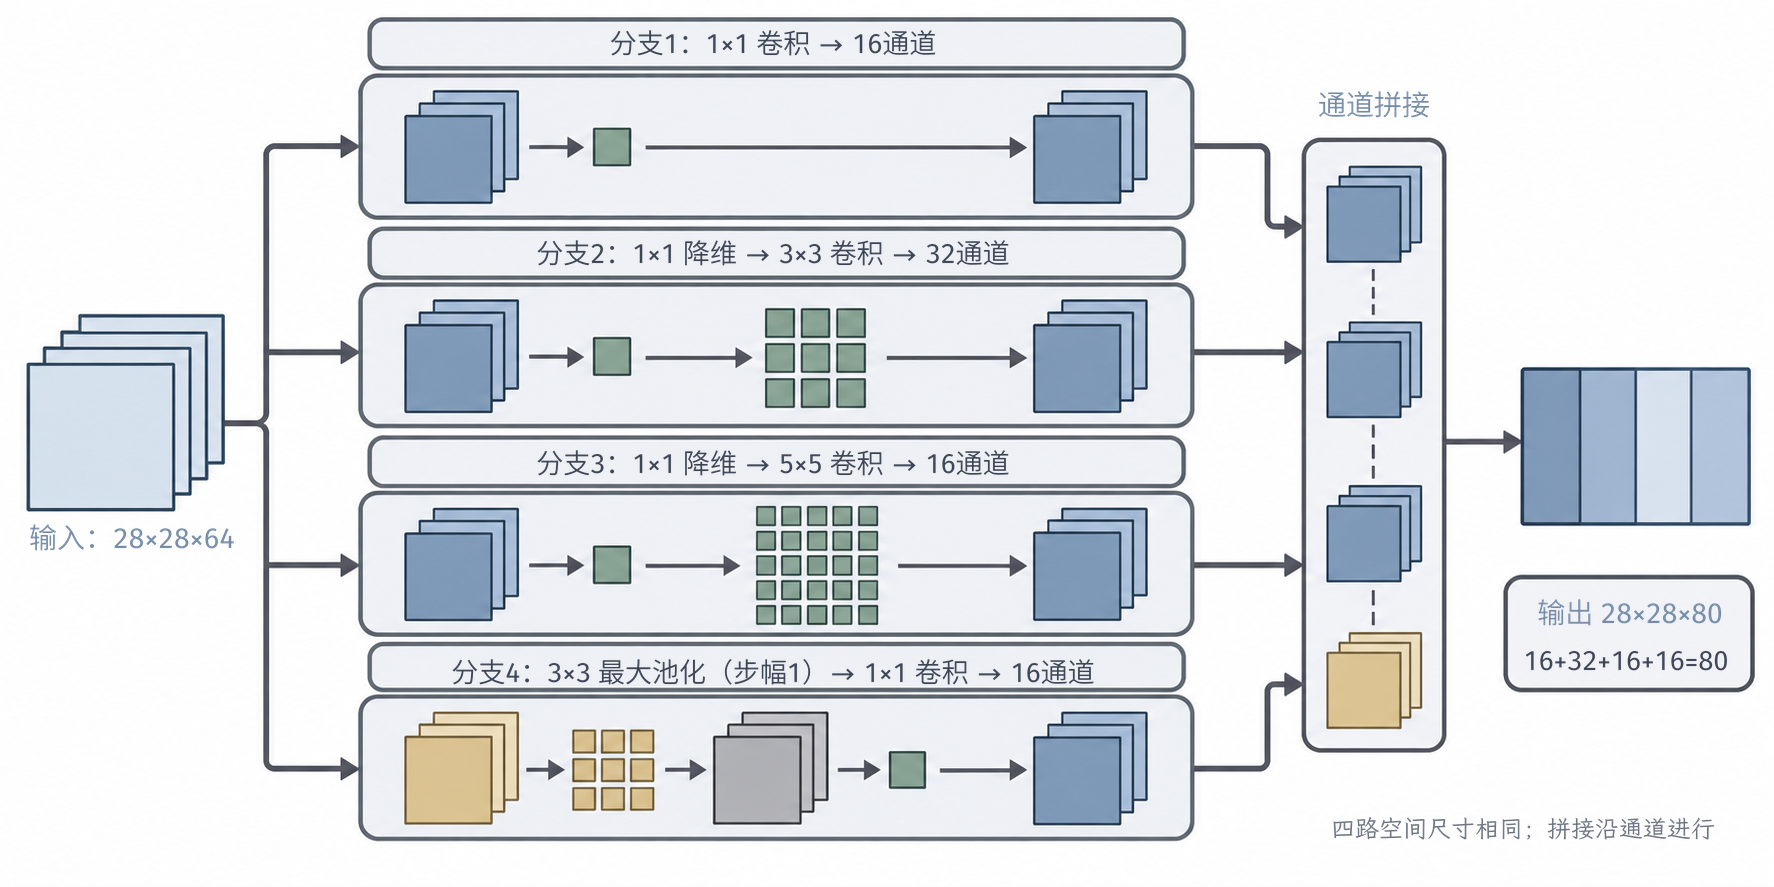
\includegraphics[width=150.199mm]{figures/05-neural-network-models/00-shared/generated/cnn-inception/figure.png}
  \caption{一个Inception模块的四分支教学配置。输入为$28\times28\times64$；四条分支分别输出16、32、16、16个通道，保持同一空间尺度，拼接得到$28\times28\times80$。中间的逐点卷积先压缩通道，最大池化采用步长一及same填充。圆角方框表示处理算子，各分支的标签给出核尺寸或通道数；右侧拼接框沿通道合并四路输出。四条路径实际并行，激活省略。}
  \label{fig:cnn-inception}
\end{figure*}

图中$3\times3$分支先将通道从64压到16，再输出32个通道，权重数为$64\times16+9\times16\times32=5632$；直接从64映射到32需要$18432$个。节省来自中间通道压缩，压缩也会限制该分支的表示。拼接保留分支间的区别，没有像相加那样把对应通道混合；后续卷积再学习如何组合这些通道。

可以固定一个空间位置，追踪四条分支怎样组成它的输出。逐点分支给出16个只在该位置混合通道的响应，另外两条卷积分支给出32个和16个结合周围位置的响应，池化分支再给出16个局部汇聚后的响应。拼接把这四组数依次放入一个80维向量。所有分支处理的是同一张空间网格，并未把图像分成四块；它们分配的是不同处理方式的通道数。下一模块的逐点卷积可以同时读取这80个数，学习哪些尺度的响应需要共同使用。

经典GoogLeNet先用普通卷积与池化形成$28\times28\times192$特征，再堆叠九个Inception模块，按两、五、两个模块分成三个尺度阶段；两个阶段间池化将空间降为14和7。末端$7\times7\times1024$特征经全局平均池化形成1024维向量，再作1000类分类。训练时，在中间层加入辅助分类器，让较浅位置也收到任务损失；推理时使用主分类路径。图~\ref{fig:cnn-googlenet}展示主路径，原论文按最长路径计22个带参数层，一个Inception模块内部则包含多条路径和多个卷积。

\begin{figure*}[htb]
  \centering
  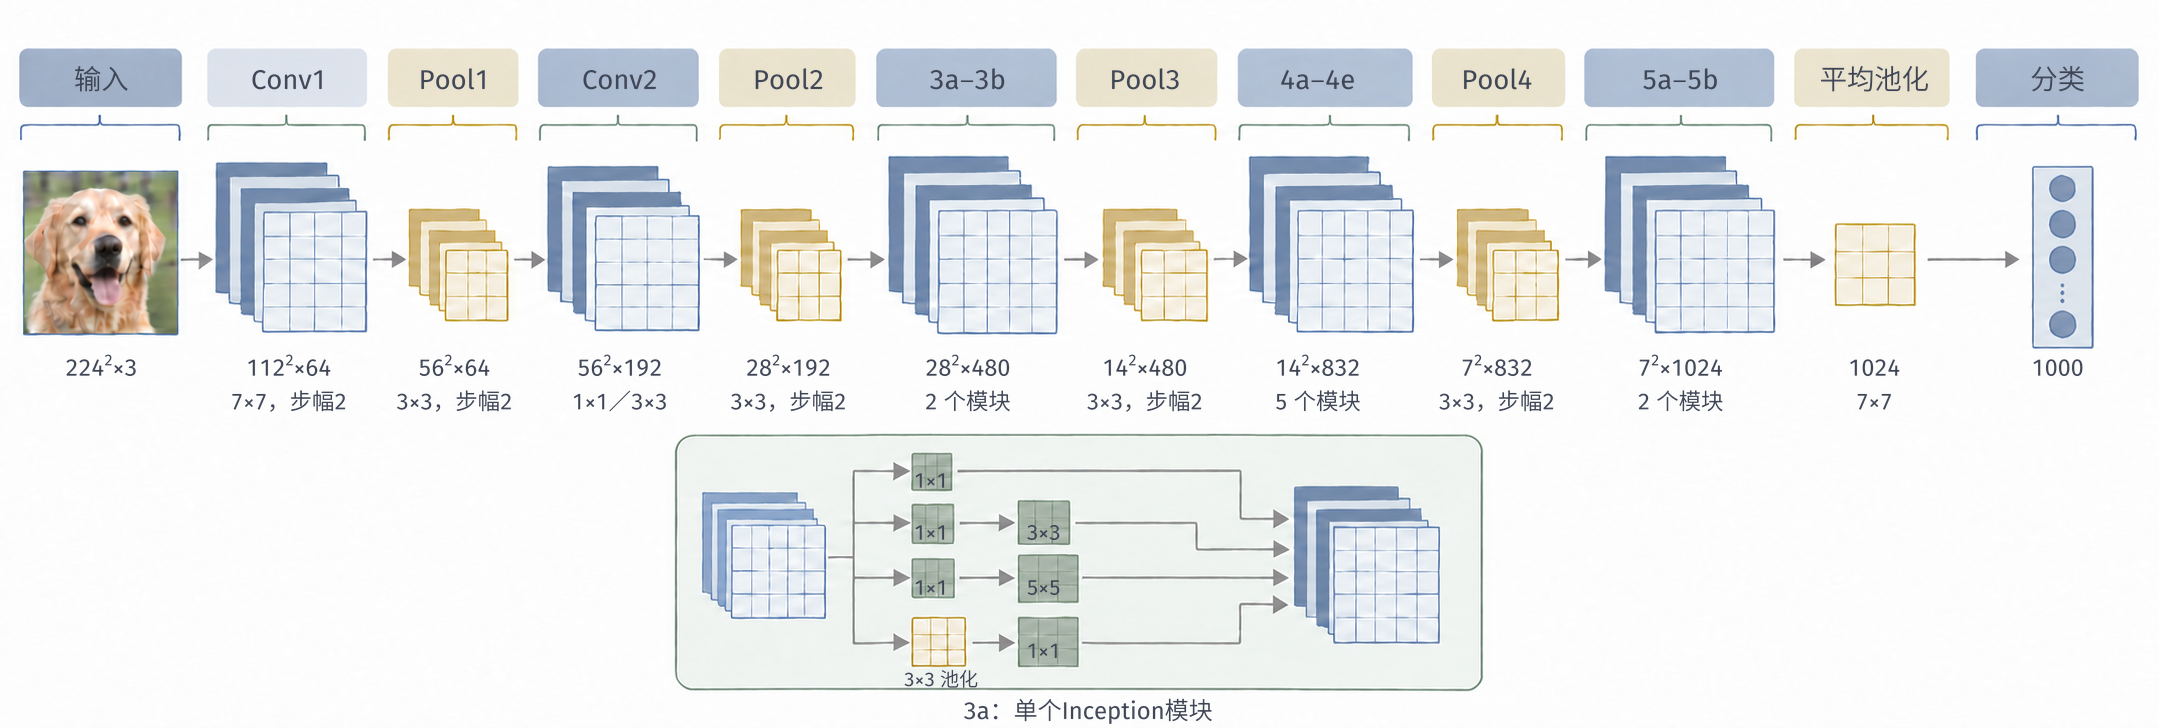
\includegraphics[width=169.000mm]{figures/05-neural-network-models/00-shared/generated/cnn-googlenet/figure.png}
  \caption{经典GoogLeNet的主分类路径。卷积前端把$224\times224$输入变成$28\times28\times192$；两个、五个、两个Inception模块组成三个阶段，阶段间池化改变空间尺度。各阶段末的通道数为480、832和1024，全局平均池化后接1000类分类器。辅助分类分支省略，下方以3a为代表展开单个Inception模块的四分支组织，主链的3a--3b组实际包含两个模块；分支机制见图~\ref{fig:cnn-inception}。}
  \label{fig:cnn-googlenet}
\end{figure*}

末端的全局平均池化还改变了分类层怎样使用位置。每个通道在$7\times7$网格上的49个响应先取平均，分类层只读取1024个通道均值。忽略偏置，这个1000类分类层有$1024\times1000$个权重；若把同一特征张量展平后直接接1000类输出，则需$49\times1024\times1000$个权重。减少来自先汇聚空间位置，但这种读出也舍去了同一通道内响应的具体位置：交换这些位置不会改变通道均值。网络须在汇聚前把分类所需的空间关系转化为通道响应；若任务本身需要逐位置答案，就应保留空间输出。

GoogLeNet用多分支增加同层处理方式，用逐点卷积控制大核分支的成本，并以全局汇聚替代庞大的全连接尾部。代价是分支调度、拼接和更多中间特征，理论乘加预算仍需结合实现分析\scite{szegedy2015googlenet}表~\ref{tab:cnn-classic-architectures}把四种架构放回共同的问题：它们如何从局部形成整体表示，又将计算与参数放在何处。

\begin{table*}[htb]
  \centering
  \begin{tabularx}{\linewidth}{@{}lXX@{}}
    \toprule
    架构 & 主体组织 & 理解结构时的侧重点\\
    \midrule
    LeNet & 卷积与可学习降采样交替 & 局部到整体；部分连接及原始输出约定\\
    AlexNet & 五个卷积层与较大全连接尾部 & 通道容量、训练机制、GPU分组及尾部成本\\
    VGG & 连续小核，阶段间池化 & 感受野、深度、规则结构及活动值成本\\
    GoogLeNet & 多尺度分支、通道压缩与拼接 & 同层并行处理、计算预算与整体汇聚\\
    \bottomrule
  \end{tabularx}
  \caption{经典卷积网络的组织方式。各行比较计算结构，没有在不同训练设置之间比较准确率。层数、输入形状和读出方式均应结合具体版本理解。}
  \label{tab:cnn-classic-architectures}
\end{table*}

\FloatBarrier

\section{参数学习}
\label{sec:cnn-learning}

卷积网络仍按前章的链式法则学习。结构带来的区别是：一个核权重在许多位置出现，一个输入又可能被多个窗口读取。因此，初始化应按局部连接数定尺度，反向传播则必须汇总所有重复使用的贡献。

\subsection{参数初始化}
\label{sec:cnn-initialization}

初始化的两个目标（打破对称、控制尺度）与前章完全相同，区别只在于卷积层里“一个单元读取多少个输入”的计数方式变了。在全连接层中，一个隐藏单元读取上一层的全部$d_{\ell-1}$个输出；而在卷积层中，一个输出位置只读取一个$k_h\times k_w$空间窗口、横跨全部$c_{\mathrm{in}}$个输入通道，因此它的局部输入数是$k_hk_wc_{\mathrm{in}}$，而不是整张图的像素数。初始化的方差应当按这个局部连接数来定。对普通卷积，通常取
\begin{equation}
  \mathrm{fan\text{-}in}=k_hk_wc_{\mathrm{in}},\qquad
  \mathrm{fan\text{-}out}=k_hk_wc_{\mathrm{out}}\text{。}
  \label{eq:cnn-fans}
\end{equation}
后者按内部位置、步长为一的连接估计，每个输入向多个输出位置及通道贡献；边界、跨步和分组会改变实际连接数。初始化实现一般采用固定的核级约定，应区分这一约定与每个位置的精确计数。

设初始权重独立、零均值、方差为$v$，与输入独立，偏置为零，各输入元素二阶矩为$q$。不同权重的交叉项均值为零，即使相邻像素相关，仍可在这个初始化模型下得到
\[
  \mathbb E[z_{i,j,o}^2]=k_hk_wc_{\mathrm{in}}vq
\]
用于内部位置的尺度估计。若预激活分布关于零对称，ReLU截去负半轴会使二阶矩减半，所以前向He初始化取
\begin{equation}
  w_{a,b,c,o}\sim\mathcal N\!\left(0,
          \frac{2}{k_hk_wc_{\mathrm{in}}}\right)\text{。}
  \label{eq:cnn-he-initialization}
\end{equation}
这与前章一致，分母变为局部输入连接数，而非整张图像的像素数。偏置可以初始化为零；不同核仍需要不同的随机权重，以打破输出通道之间的对称性\scite{he2015rectifiers}

对中心附近近似单位斜率的激活，Glorot初始化可用方差$2/(\mathrm{fan\text{-}in}+\mathrm{fan\text{-}out})$折中前后向尺度。分组层的局部fan-in需除以组数；只有一个空间核的逐通道层，每个输出读取$k_hk_w$个值。跨步卷积中，每个输入参与的输出窗口更少且可能随位置变化，简单独立性估计也不会捕捉共享权重造成的空间相关。初始化提供的是起始尺度依据，训练中还需检查实际活动值与梯度，不能把这些近似当成全过程保证。

\subsection{卷积层反向传播}
\label{sec:cnn-backpropagation}

卷积的前向计算理解之后，反向传播只需抓住“共享”带来的两个镜像现象，它们都可以直接用前章的链式法则推出，不必记忆新公式。

\emph{第一，核权重在许多位置被重复使用，所以它的梯度要沿位置累加。}同一个权重$w_{a,b,c,o}$既出现在左上角的窗口里，也出现在右下角的窗口里；它对损失的总影响等于它在每个使用位置上的局部影响之和。

\emph{第二，一个输入像素会被多个重叠窗口读取，所以它的梯度也要沿窗口累加。}一个内部像素可能同时属于若干相邻窗口，每个窗口都把自己的一部分梯度通过该像素对应的核权重传回来，这些贡献要叠加到同一个输入上。

下面把这两点写成公式。以式\eqref{eq:cnn-batch-objective}的批平均损失$L_B$为求导对象，记上游传到卷积预激活的梯度为$\delta_{t,i,j,o}=\partial L_B/\partial z_{t,i,j,o}$，其中$t\in B$。这个导数包含整批所有损失项的影响，不只是样本$t$自身的损失。若已知的是紧接卷积的激活输出梯度，需先乘$\sigma'(z_{t,i,j,o})$；若中间还有归一化，则按前向相反顺序对其求导。特别是训练态BN，必须经过完整批统计量的计算图，才能取得这里的$\delta$。以下采用式\eqref{eq:cnn-layer-forward}，并固定零填充约定。

先看第一点。同一权重$w_{a,b,c,o}$在各样本及各输出位置重复使用，因此链式法则给出
\begin{equation}
  \begin{aligned}
    \frac{\partial L_B}{\partial w_{a,b,c,o}}
      &=\sum_{t\in B}\sum_{i=0}^{h'-1}\sum_{j=0}^{w'-1}
         \delta_{t,i,j,o}\widetilde x_{t,u(i,a),v(j,b),c},\\
    \frac{\partial L_B}{\partial b_o}
      &=\sum_{t\in B}\sum_{i=0}^{h'-1}\sum_{j=0}^{w'-1}
         \delta_{t,i,j,o}\text{。}
  \end{aligned}
  \label{eq:cnn-parameter-gradients}
\end{equation}
每次使用该权重都会产生一项局部导数，共享参数的总导数就是这些项之和。不同位置的贡献可以相互加强，也可以抵消；参数共享并不要求所有位置产生相同响应或相同梯度。这里$\delta$已包含批平均的$1/|B|$，汇总时不再除以批量大小。只有前向映射逐样本独立时，才可先由单样本损失分别求导，再在批量上平均。

一个卷积输入$x_{t,u,v,c}$可能参与本样本的多个输出窗口，也可能连接多个输出通道。将卷积局部映射中所有包含它的项找出，得到
\begin{equation}
  \frac{\partial L_B}{\partial x_{t,u,v,c}}
  =\sum_{i,j,o}\sum_{a,b}
    \delta_{t,i,j,o}w_{a,b,c,o}
    \mathbb I\{u=u(i,a),\ v=v(j,b)\}\text{。}
  \label{eq:cnn-input-gradient}
\end{equation}
其中$u,v$在原输入范围内，$\mathbb I$为条件成立时取一的指示函数，求和范围沿用前向计算。索引条件直接选出前向读取了该坐标的项，因此也适用于跨步和空洞。若使用复制或反射填充，一个原输入还可能对应多个扩展位置，需把这些位置的梯度再累加回来；其索引累积关系随填充映射改变。

矩阵形式揭示了它与转置卷积的联系。固定参数时，将每个样本的张量展平，前向预激活为$\bm z_t=\bm C\bm x_t+\bm b_{\mathrm{rep}}$，$\bm b_{\mathrm{rep}}$表示各位置重复的偏置；把$\delta_{t,i,j,o}$展平为$\bm\delta_t$，就有
\begin{equation}
  \nabla_{\bm x_t}L_B=\bm C^\top\bm\delta_t\text{。}
  \label{eq:cnn-backprop-transpose}
\end{equation}
输入梯度正是前向线性算子的转置作用。数据展开实现则先把每个窗口的梯度算出来，再把各列放回输入坐标，并累加重叠部分；这个回填步骤常称为col2im，同一输入坐标对应的窗口梯度在此相加。

仍用式\eqref{eq:cnn-matrix-example}，取仅含这一个输入的批量，不加归一化、不填充、步长一，令$L_B$为全部互相关输出之和。九个输出的$\delta$均为一，则
\begin{equation}
  \nabla_{\bm K}L_B=
    \begin{bmatrix}54&63\\90&99\end{bmatrix},\qquad
  \nabla_{\bm X}L_B=
    \begin{bmatrix}
      1&1&1&0\\1&0&0&-1\\1&0&0&-1\\0&-1&-1&-1
    \end{bmatrix}\text{。}
  \label{eq:cnn-gradient-example}
\end{equation}
例如左上核权重汇总九个窗口的左上元素，和为$54$；$x_{1,1}=6$既以系数$1$参与一个窗口，也以系数$-1$参与另一个窗口，两项相消。虽然某些核权重当前为零，它们的梯度仍可非零，因为改变该权重会立即改变相应输出。偏置梯度为$9$。这个例子把“共享参数累积”与“重叠输入累积”区分开来。

图~\ref{fig:cnn-backprop-shared-overlap}在同一输入与共享核上展开这两种累积。左侧按核坐标收集窗口贡献，右侧按输入坐标收集读取该位置的贡献。

\begin{figure*}[htbp]
  \centering
  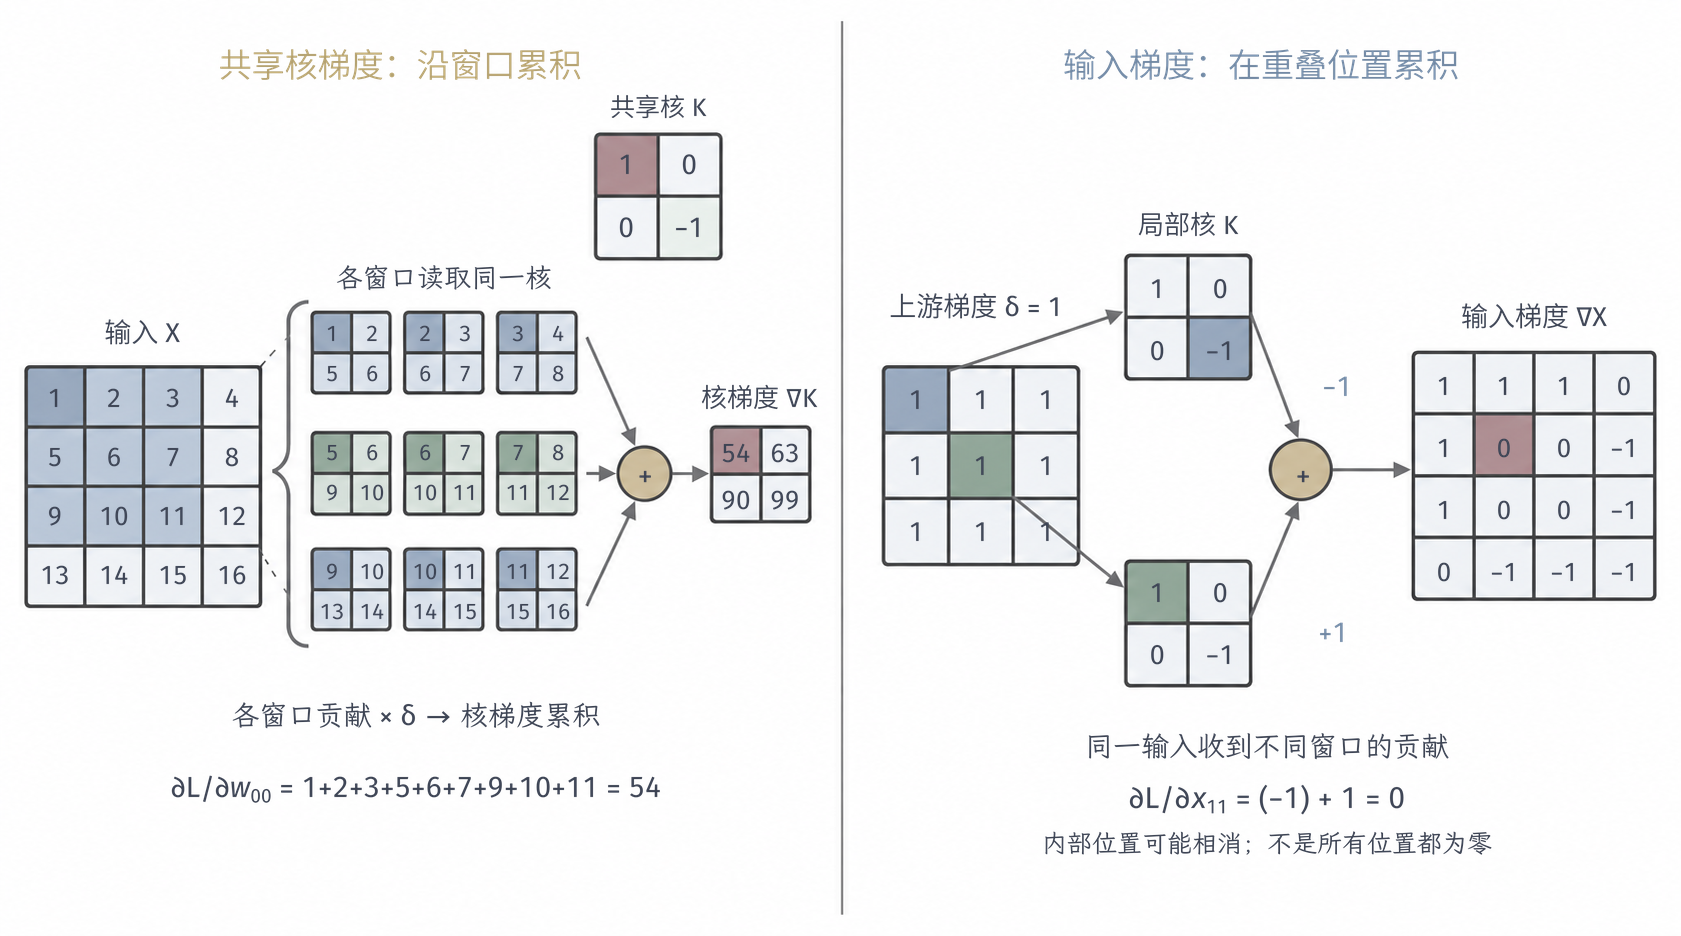
\includegraphics[width=142.325mm]{figures/05-neural-network-models/00-shared/generated/cnn-backprop-shared-overlap/figure.png}
  \caption{式~\eqref{eq:cnn-gradient-example}中的两种梯度累积。输入为按行排列$1$至$16$的$4\times4$矩阵，核为$(1,0;0,-1)$，步长一、无填充，损失为九个输出之和。左图汇总九个窗口对同一核参数的贡献；右图突出$x_{1,1}=6$的两项非零贡献，二者相消；另两项贡献因对应核值为零而为零。}
  \label{fig:cnn-backprop-shared-overlap}
\end{figure*}

\subsection{池化层反向传播}
\label{sec:cnn-pooling-backpropagation}

池化没有标准的可学习参数，但它决定上游梯度怎样返回输入。仍对完整批损失求导，设池化输出的梯度为$g_{t,i,j,c}=\partial L_B/\partial y_{t,i,j,c}$。平均池化对每个参与的元素具有相同导数，因此
\begin{equation}
  \frac{\partial L_B}{\partial x_{t,u,v,c}}
  =\sum_{i,j}\frac{g_{t,i,j,c}}{q_{i,j}}
                  \mathbb I\{(u,v)\in\Omega_{i,j}\}\text{。}
  \label{eq:cnn-average-pooling-gradient}
\end{equation}
分母必须与前向平均采用的计数相同。窗口重叠时，一个输入收到多项；全局平均池化则将某通道的上游梯度均分给该通道全部位置。

最大池化在最大值唯一时，只对被选中的元素有非零导数。前向计算记录其位置$(u^*_{t,i,j,c},v^*_{t,i,j,c})$，后向使用同一位置：
\begin{equation}
  \frac{\partial L_B}{\partial x_{t,u,v,c}}
  =\sum_{i,j}g_{t,i,j,c}
       \mathbb I\{(u,v)=(u^*_{t,i,j,c},v^*_{t,i,j,c})\}\text{。}
  \label{eq:cnn-max-pooling-gradient}
\end{equation}
若多个元素并列最大，函数在该点不可微；实现可以按固定规则选择一个位置，也可以采用最大值集合上的合法次梯度分配。后向采用与前向对应的选择或次梯度规则。同一元素若是多个重叠窗口的最大值，会收到这些窗口梯度的和。

对式\eqref{eq:cnn-pooling-example}，令四个输出梯度均为一。平均池化使每个输入收到$1/4$，最大池化只让原矩阵中的$6,8,14,16$各收到$1$。回传规则因此保留了两种汇聚方式的区别：平均把影响均分，最大把影响路由到当前胜出的位置。卷积与池化梯度接入前章的反向传播后，就能联合更新整个网络；优化器和学习率的通用选择由后续训练章讨论。

\section{卷积神经网络的扩展}
\label{sec:cnn-extensions}

\subsection{支持更深的网络结构}
\label{sec:cnn-deep-structures}

到VGG为止，增加深度的主要手段是不断串联卷积层。但实践中发现一个反直觉的现象：当网络从几十层继续加深时，\emph{训练误差不降反升}。这不能用过拟合解释——过拟合是训练误差很低、测试误差升高；这里连训练集上的误差都变差了，说明瓶颈在优化本身：层数过多后，梯度在长长的串联链路上反复相乘，深层参数难以获得有效的更新信号。这一现象称为\term{退化问题}（degradation problem），它发生在训练集上，是更深参数化带来的求解困难，而非单纯的泛化问题。ResNet论文在其图像实验中报告并研究了这一现象\scite{he2016resnet}

一个自然的破解思路是：\emph{不要强迫每一叠层都去重新构造完整的表示，而是允许信息“抄近道”直接绕过它们}。如果新加入的几层在当前任务上暂时没有用处，最理想的情况是它们能轻松地退化为“什么都不改”，网络的表现至少不应比更浅时更差。跨层连接正是提供这种近道的机制。下面比较三种组织方式：把旁路信息与变换结果直接\emph{相加}（残差连接）、用一个可学习的\emph{门}控制新旧信息的混合比例（Highway网络），以及把旧特征沿通道轴\emph{拼接}保留下来（密集连接）。它们都不形成有向环，因而仍是前馈网络，但各自改变了中间表示和梯度回传的路径。

\subsubsection{残差连接与ResNet}
\label{sec:cnn-resnet}

先看“让多余的层能轻松什么都不改”在数学上意味着什么。普通串联模块要把输入$\bm x$映射成目标输出$\bm y=\bm H(\bm x)$；若理想的$\bm H$恰好接近恒等（即这几层本可不改变输入），普通模块就必须\emph{主动学出}恒等映射$\bm H(\bm x)=\bm x$，而用一堆带非线性的卷积层精确凑出恒等相当困难。\term{残差连接}（residual connection）换了一个参数化：把输入直接加到变换分支的输出上，让这组层只需要学习“输出相对输入还差多少”。将输入特征展平为$\bm x\in\mathbb R^d$，维度相同时，模块写为
\begin{equation}
  \bm y=\bm x+\bm F_{\bm\theta}(\bm x)\text{。}
  \label{eq:cnn-residual-block}
\end{equation}
其中$\bm F_{\bm\theta}:\mathbb R^d\to\mathbb R^d$由若干卷积、归一化和激活组成。若目标映射接近恒等，残差分支只需接近零。这里的“残差”是模块输出相对于输入的差，不是标签减去预测值的训练误差。

图~\ref{fig:cnn-resnet}展开一个基本模块中的层与残差连接。上方旁路把输入直接送到加法节点，主分支则计算需要叠加的变换；图中的模块还在相加后施加一次ReLU。
\begin{figure*}[htbp]
  \centering
  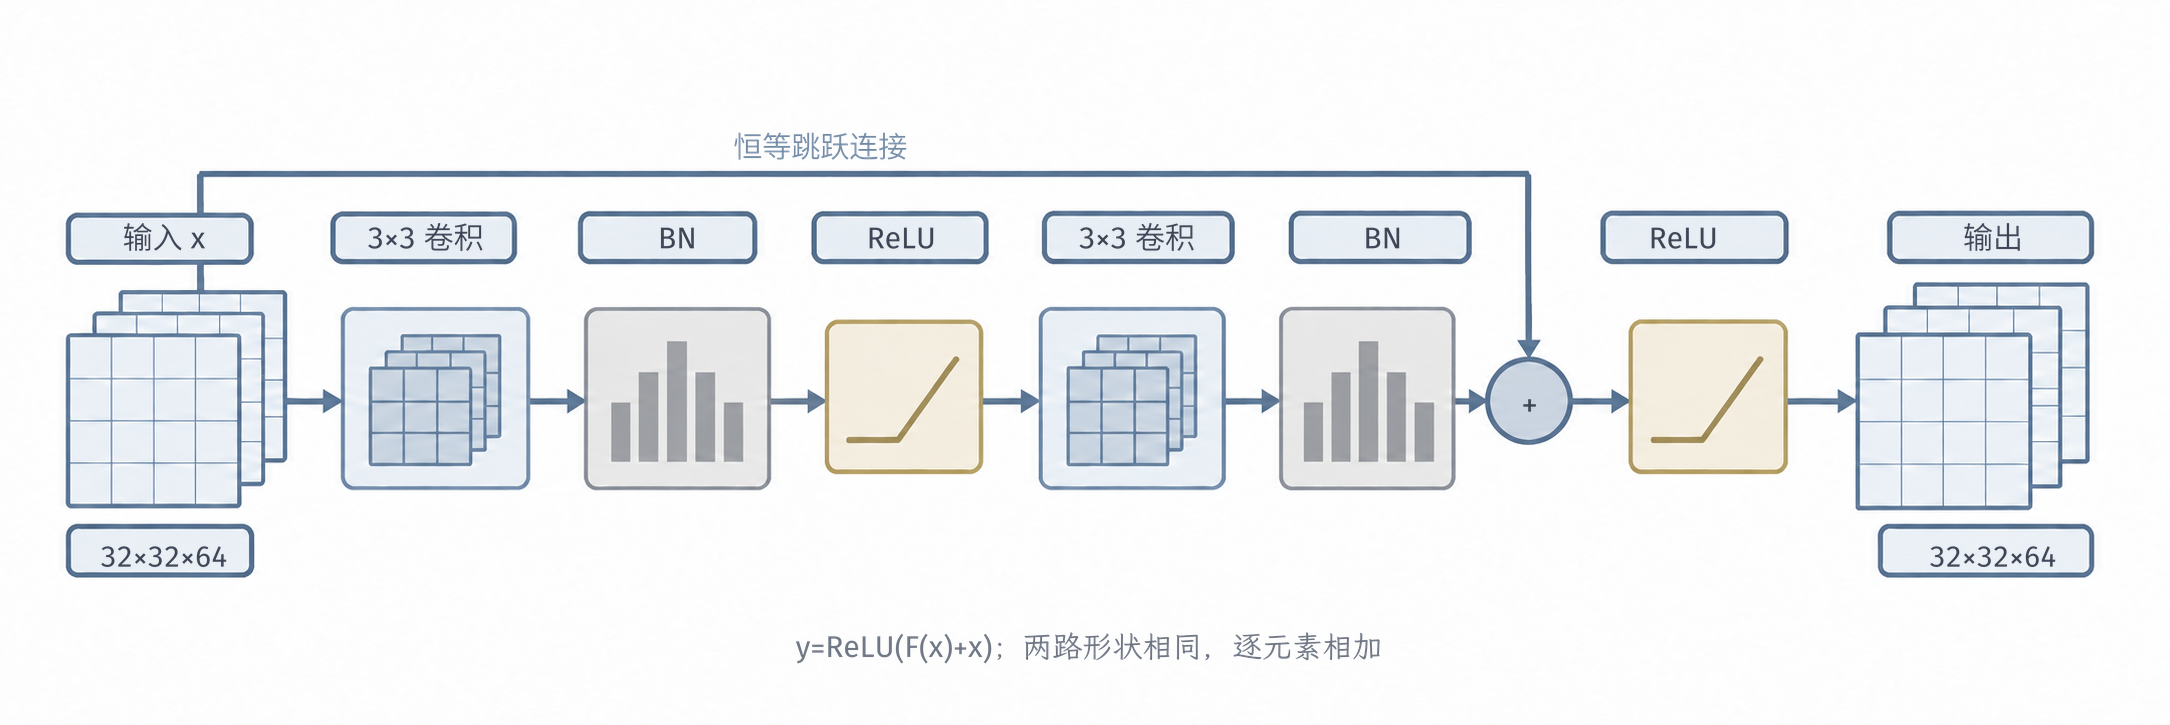
\includegraphics[width=169.000mm]{figures/05-neural-network-models/00-shared/generated/cnn-resnet/figure.png}
  \caption{残差基本模块中的逐层变换与恒等旁路。主分支依次经过$3\times3$卷积、BN、ReLU及第二个$3\times3$卷积、BN，再与直接传来的输入逐元素相加并激活。两次卷积均保持$32\times32\times64$形状，上方旁路跳过主分支的变换。圆角方框表示算子，圆形加号节点表示逐元素相加；改变尺度或通道时，旁路需要投影。}
  \label{fig:cnn-resnet}
\end{figure*}
下面只考察相加本身，暂不在相加后施加额外激活；含训练态BN时，$\bm x$应包含参与统计的整批特征。在可微位置，令$\bm J_F=\partial\bm F/\partial\bm x$。输入的微小变化$\mathrm d\bm x$沿两条路径分别产生$\mathrm d\bm x$与$\bm J_F\,\mathrm d\bm x$，相加后有
\[
  \mathrm d\bm y=\mathrm d\bm x+\bm J_F\,\mathrm d\bm x
    =(\bm I+\bm J_F)\,\mathrm d\bm x\text{。}
\]
对标量损失$\ell$，链式法则给出$\mathrm d\ell=(\nabla_{\bm y}\ell)^\top\mathrm d\bm y$。代入上式，再与$\mathrm d\ell=(\nabla_{\bm x}\ell)^\top\mathrm d\bm x$比较，就得到
\begin{equation}
  \begin{aligned}
    \frac{\partial\bm y}{\partial\bm x}&=\bm I+\bm J_F,\\
    \nabla_{\bm x}\ell&=(\bm I+\bm J_F)^\top\nabla_{\bm y}\ell\\
      &=\nabla_{\bm y}\ell+\bm J_F^\top\nabla_{\bm y}\ell\text{。}
  \end{aligned}
  \label{eq:cnn-residual-gradient}
\end{equation}
末行的第一项直接经过恒等路径，第二项经过残差分支。两项共同决定输入梯度，例如标量分支$F(x)=-x$就有$1+F'(x)=0$，两路贡献恰好相消。多块连乘后，尺度还随各块Jacobian矩阵变化；恒等路径改变了传播结构，整体梯度仍由全部路径决定。

若记相加结果为$\bm z=\bm x+\bm F(\bm x)$，再令$\bm y=\operatorname{ReLU}(\bm z)$，则反向还要先经过ReLU：
\[
  \nabla_{\bm x}\ell
    =(\bm I+\bm J_F)^\top\bm D_{\mathrm{ReLU}}\nabla_{\bm y}\ell\text{。}
\]
在$z_i\neq0$处，$\bm D_{\mathrm{ReLU}}$的第$i$个对角元素为$\mathbb I\{z_i>0\}$；零点按实现选定导数。这层激活也筛选恒等路径传来的贡献，相加结果与最终输出因而具有不同的导数。

当阶段间下采样或改变通道时，输入与分支结果不能直接逐元素相加。可用投影$\bm P$调整形状，写为$\bm y=\bm P\bm x+\bm F(\bm x)$；例如用跨步$1\times1$卷积同时改变空间尺寸与通道。此时跨层路径的Jacobian矩阵是$\bm P$，不再是$\bm I$，合并输出的Jacobian矩阵相应变为$\bm P+\bm J_F$。选择恒等或投影，取决于两条分支的形状和希望保留的映射。

ResNet在多个阶段堆叠残差模块。基本模块常用两个$3\times3$卷积；瓶颈模块用$1\times1$压缩通道、$3\times3$处理空间、再用$1\times1$恢复通道，以控制主体计算。经典版本在相加后使用激活。不同版本通过激活位置、旁路投影和下采样所在分支确定计算图；这些选择共同影响信息和梯度路径。

ResNet-18的主干分为四个阶段：对$224\times224$输入，前端$7\times7$卷积取步长二、填充三，产生$112\times112$特征；接BN、ReLU及$3\times3$、步长二、填充一的最大池化，得到$56\times56$网格。四个阶段分别使用64、128、256、512个通道，每个阶段包含两个基本模块；后三阶段的首模块将空间减半，并用投影匹配相加形状。末端全局平均池化与分类层完成整体读出。

\subsubsection{门控连接与Highway网络}
\label{sec:cnn-highway}

直接相加始终保留输入并叠加变换；若希望根据当前输入控制两条路径的比例，可以让网络学习一个门。\term{Highway网络}（Highway network）用控制门调节哪些坐标更多采用新变换、哪些更多保留原值。维度相同、保留门与变换门互补时，
\begin{equation}
  \begin{aligned}
    \bm g(\bm x)&=\operatorname{Sigmoid}(\bm G(\bm x)),\\
    \bm y&=\bm g(\bm x)\odot\bm F(\bm x)
            +(\bm1-\bm g(\bm x))\odot\bm x\text{。}
  \end{aligned}
  \label{eq:cnn-highway-block}
\end{equation}
其中$\bm F$为变换路径，$\bm G$产生与输入同形状的门得分，Sigmoid逐元素把门值限制在$(0,1)$。在卷积模块中，$\bm F$和$\bm G$都可使用共享局部计算。门值接近零时以保留路径为主，接近一时以变换路径为主。原工作采用负的门偏置，使初始门倾向保留输入，帮助很深的网络开始学习\scite{srivastava2015highway}

门值随输入变化，这一变化也参与输出导数。
在可微位置，先固定一个坐标$i$，将式\eqref{eq:cnn-highway-block}写成$y_i=g_iF_i+(1-g_i)x_i$；这里$g_i$和$F_i$都随整个输入$\bm x$变化。对两个乘积分别使用乘积法则，有
\[
  \begin{aligned}
    \mathrm d y_i
      &=g_i\,\mathrm d F_i+F_i\,\mathrm d g_i
        +(1-g_i)\,\mathrm d x_i-x_i\,\mathrm d g_i\\
      &=g_i\,\mathrm d F_i+(1-g_i)\,\mathrm d x_i
        +(F_i-x_i)\,\mathrm d g_i\text{。}
  \end{aligned}
\]
第一项记录变换结果的变化，第二项记录保留输入的变化，第三项合并了同一个门同时调整两条路径的影响。把所有坐标叠成向量，代入$\mathrm d\bm F=\bm J_F\,\mathrm d\bm x$和$\mathrm d\bm g=\bm J_g\,\mathrm d\bm x$，其中$\bm J_F=\partial\bm F/\partial\bm x$、$\bm J_g=\partial\bm g/\partial\bm x$，即可把每类逐坐标缩放写成一个对角矩阵。
记$\operatorname{Diag}(\bm v)$为以向量$\bm v$作对角线的矩阵，$\bm J_g$为门的Jacobian矩阵，则
\begin{equation}
  \begin{aligned}
    \bm J_y={}&\operatorname{Diag}(\bm g)\bm J_F
      +\operatorname{Diag}(\bm1-\bm g)\\
      &+\operatorname{Diag}(\bm F(\bm x)-\bm x)\bm J_g\text{。}
  \end{aligned}
  \label{eq:cnn-highway-gradient}
\end{equation}
末项来自门值随输入变化的影响。负偏置使门初始更接近保留路径，也可能让Sigmoid进入导数较小的区域，门参数的学习仍需合适尺度。Highway增加了可学习的路由及其参数成本；式\eqref{eq:cnn-highway-block}中两条系数之和为一，与ResNet无门控的直接相加具有不同约束。

图~\ref{fig:cnn-highway}展开变换、门和保留路径，两个逐元素乘法节点分别调节变换结果与原输入，再由相加节点合并。三条路径都保持$h\times w\times c$形状，门按位置和通道决定缩放系数；改变形状的模块还要为保留路径安排投影，并使门与两路结果具有匹配的目标形状。

\begin{figure*}[htb]
  \centering
  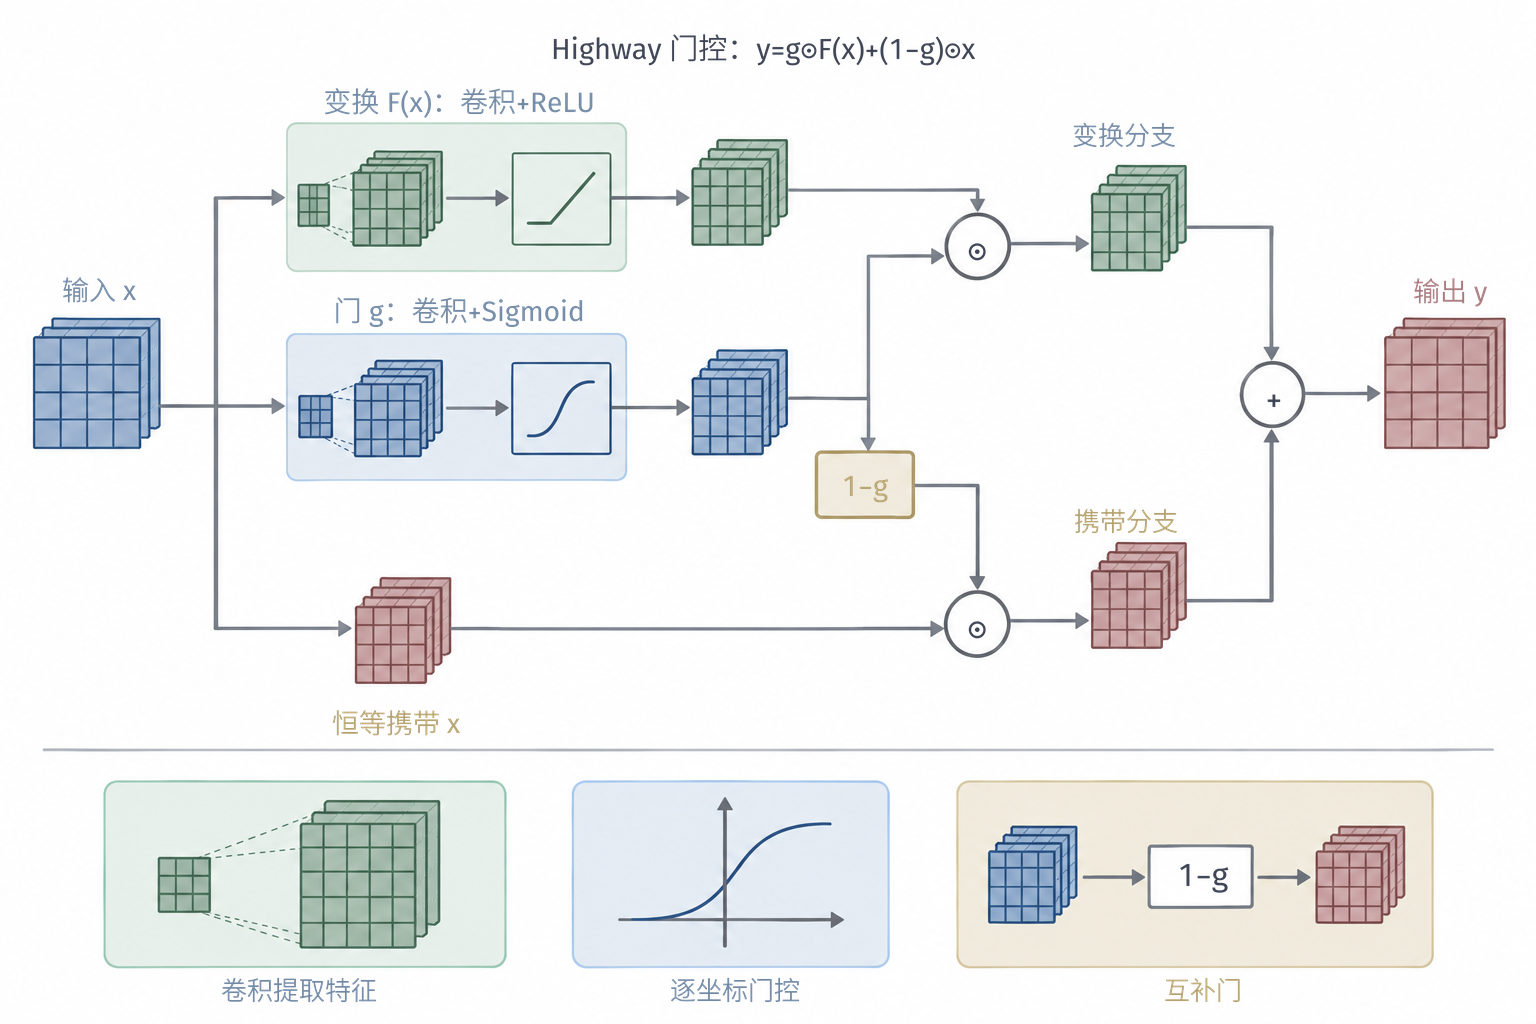
\includegraphics[width=130.048mm]{figures/05-neural-network-models/00-shared/generated/cnn-highway/figure.png}
  \caption{同形状卷积Highway模块。上方卷积与ReLU产生$\bm F(\bm x)$，门路径经卷积与Sigmoid产生$\bm g$，保留路径传递原输入；两个$\odot$节点分别计算$\bm g\odot\bm F(\bm x)$和$(\bm1-\bm g)\odot\bm x$，再由$+$节点相加。所有特征与门具有同一空间、通道形状，圆角方框表示各条路径的处理算子。}
  \label{fig:cnn-highway}
\end{figure*}
\FloatBarrier

\subsubsection{密集连接与DenseNet}
\label{sec:cnn-densenet}

残差相加把旧特征和新特征合在相同通道中。若希望后层仍能分别读取先前各层的特征，可以沿通道轴保留它们。\term{密集连接}（dense connection）使一个块内的每层读取全部先前层的输出；DenseNet按这种方式构造卷积模块：
\begin{equation}
  \bm H^{(\ell)}=\bm F_\ell\!\left(
      [\bm H^{(0)},\bm H^{(1)},\ldots,\bm H^{(\ell-1)}]
    \right)\text{。}
  \label{eq:cnn-dense-block}
\end{equation}
方括号表示通道拼接，不是逐元素相加；块内空间高、宽必须一致。$\bm H^{(0)}$为块的输入，各层只产生新的通道，旧特征仍可供更后层直接读取\scite{huang2017densenet}

若块输入有$c_0$个通道，每层新增$k$个通道，$k$称为\term{增长率}（growth rate），即每层增加的特征数。第$\ell$层输入有$c_0+(\ell-1)k$个通道，包含$L$层的整个块输出有$c_0+Lk$个通道。以$c_0=32,k=16,L=4$为例，各层依次读取$32,48,64,80$个通道，最终拼接得到$96$个通道。块间的\term{过渡层}（transition layer）用逐点卷积压缩通道，再通过池化降低空间尺寸，限制持续增长的特征规模。

密集连接提供直接的特征读取和梯度路径，但需要保留更多活动值。若每层只用一个产生$k$个新通道的$3\times3$卷积，忽略偏置，块内权重数为
\begin{equation}
  9k\sum_{\ell=1}^{L}\bigl(c_0+(\ell-1)k\bigr)
  =9k\left(Lc_0+\frac{kL(L-1)}2\right)\text{。}
  \label{eq:cnn-dense-cost}
\end{equation}
固定增长率下，这个简化块的通道相关成本随层数呈二次增长；瓶颈和压缩设计会改变具体成本。残差模块维持相加后的通道数，密集模块保留旧通道并增加新通道，二者以不同方式复用特征，活动值内存与计算量也由各自的通道增长和模块操作决定。


图~\ref{fig:cnn-densenet}从左向右展示一个三层教学密集块：32个初始通道加上三组16个新通道，输出为80个通道。每次变换前的全部特征经旁路保留，再与本层新产生的通道拼接，因而后层仍能读取每个先前层的输出。若在块后接过渡层，可用$1\times1$卷积把80个通道压缩为40个，再通过池化把$32\times32$空间网格缩为$16\times16$。

\begin{figure*}[htb]
  \centering
  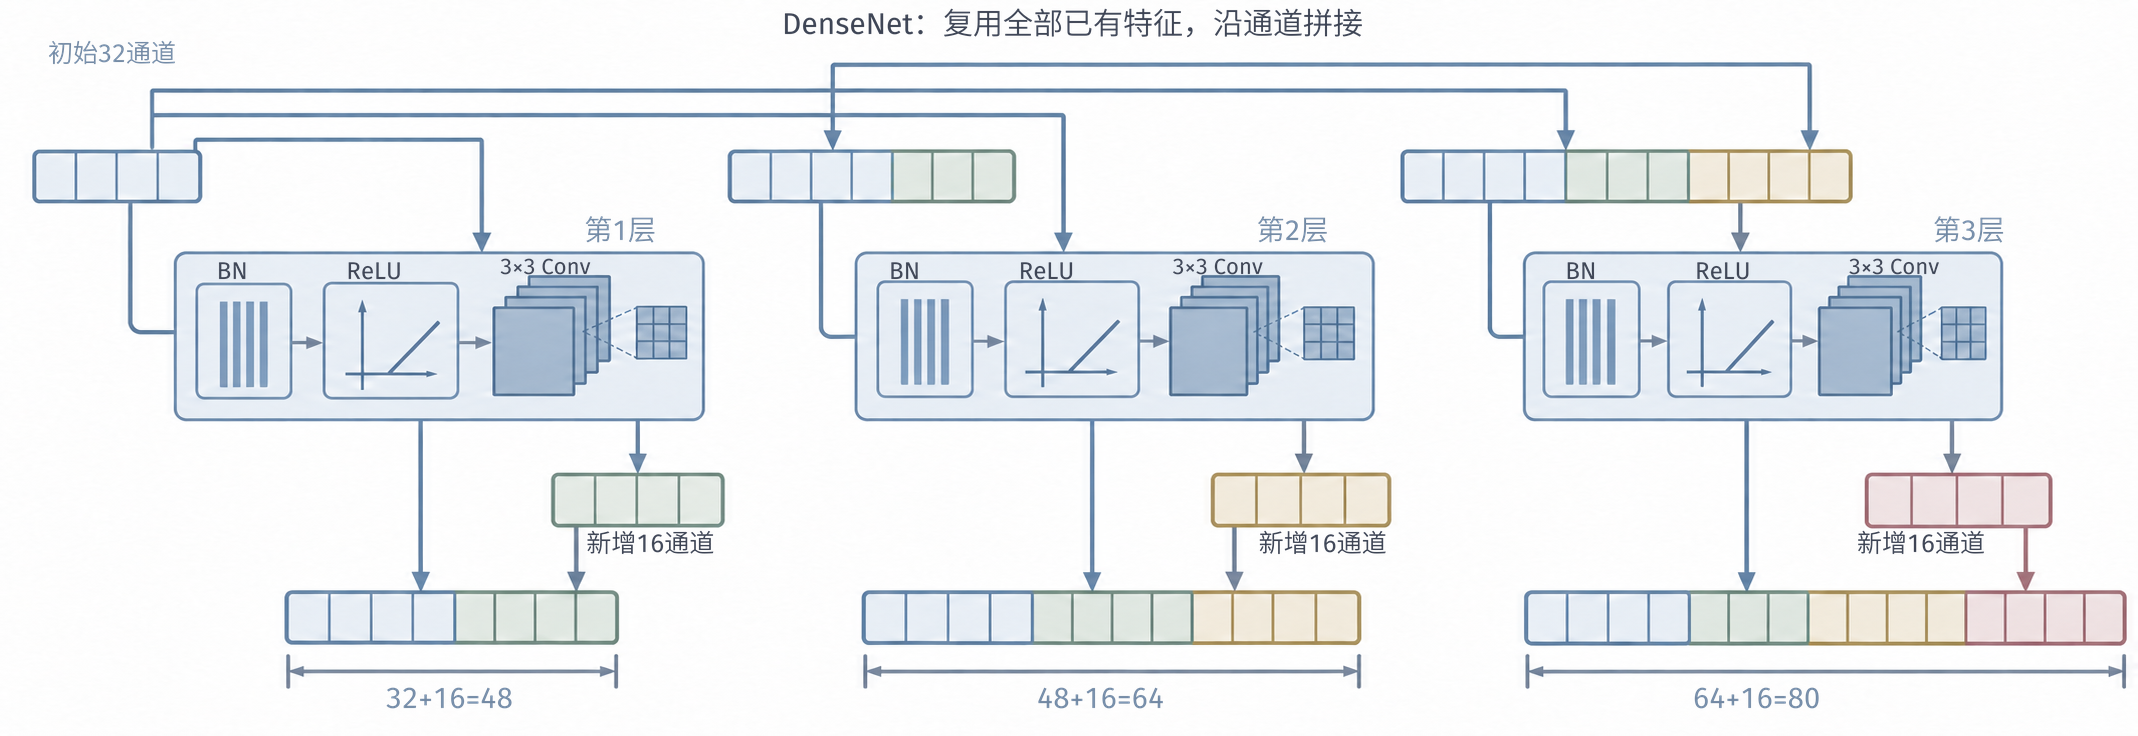
\includegraphics[width=169.000mm]{figures/05-neural-network-models/00-shared/generated/cnn-densenet/figure.png}
  \caption{DenseNet的三层教学密集块。各$\bm F_\ell$依次执行BN、ReLU和$3\times3$卷积，保持$32\times32$空间网格并新增16个通道。三次变换分别读取32、48、64个通道；上方旁路保留变换前的全部特征，标出的32、48、64为累计通道数；卷积下方的16为新增通道数。拼接位置将新旧特征沿通道合并，最终得到80个通道。逐次累积拼接等价于保留并向后传递全部先前层的输出，不作逐元素相加。}
  \label{fig:cnn-densenet}
\end{figure*}
\FloatBarrier

沿图中的第三次变换看，输入的64个通道由三部分组成：32个块输入通道、第一层新增的16个通道、第二层新增的16个通道。第三层同时读取这三组特征，但只输出自己的16个新通道；最终的80通道输出才把四组特征完整拼在一起。“读取64个通道”与“产生16个通道”分别描述该层的输入和输出，增长率只限制后者。后层可以学习重新组合旧特征，无须先在每一次相加中把旧特征与新特征合成一组。

保留旧特征也改变了反向传播的汇总位置。同一个早期特征可以同时被块内多个后层读取，损失沿这些读取路径返回的梯度，需要在这个早期特征处相加。拼接的反向操作则按通道切开输出梯度，把各段送回原来对应的特征。这些直接读取路径减少了某些梯度必须经过的串联变换数，但每条路径上的导数及其汇总仍由具体参数决定，不能据此保证梯度始终保持某个尺度。

过渡层负责结束这种持续保留。若用逐点卷积把80个通道压成40个，每个新通道都是原来80个通道的可学习组合；下一块收到的是这40组组合结果，已不再分别保留全部旧通道。随后的池化再减少空间位置。压缩比例与增长率因而需要一起选择：较小的增长率减慢块内通道增加，较强的压缩减少块间传递的特征，两者都影响后层能够读取哪些信息及其成本。

\FloatBarrier

\section{理论分析}
\label{sec:cnn-theory}

卷积、池化和跨层连接都是对候选函数施加的结构约束。约束带来了参数共享和计算效率，但任何约束都是双刃剑：它在符合数据规律时帮助学习，在不符合时则可能从根本上排除目标函数。与前章一样，本节严格区分三个不同层面的问题，避免用一个层面的结论替代另一个：\emph{表达能力}问这些结构约束是否还\textbf{允许}网络表示目标函数（结构会不会把需要的信息删掉）；\emph{收敛性}问共享参数下的梯度下降\textbf{能否}找到好参数；\emph{泛化性}问找到的参数在新图像上的\textbf{风险有多大}。泛化分析采用$n$个独立同分布训练样本及同分布测试样本，架构和参数约束在抽样前就固定；若约束是看过数据后才选择的，则还要额外计入选择代价。

\subsection{表达能力}
\label{sec:cnn-expressivity}

对卷积结构，表达能力问题有一个比全连接网络更尖锐的形式：局部连接、权值共享和下采样在利用规律的同时，也明确地\emph{丢弃}了某些信息。因此判断其表达能力，关键是看被丢弃的信息是否恰好是完成任务所必需的。如果目标是“在任何位置识别同一种平移后的图案”，局部共享与目标高度吻合；但如果任务要求不同位置必须使用不同规则（例如图像左上角和右下角的同样图案对应不同含义），共享结构就可能无法表达，除非额外提供位置特征或不同的读出方式。同样，固定大小的感受野之外的信息无法在该层直接参与判断，只有靠增加深度、加大核宽或引入全局读取来突破这一边界。

池化和下采样对表达能力的限制尤其直接：它们可能把两个\emph{不同}的输入映射成\emph{同一个}表示。一旦两个本应区分的类别被汇聚成了相同特征，后续无论再堆多少层、再怎么加宽，都只能给它们相同的输出，信息无法凭空恢复。因此一个卷积网络族的表达能力，同时取决于可学习参数和结构保留了哪些信息；位置、细节和长距离交互一旦被删除，扩大后续层也无法弥补这一限制。下面用两个定理分别从“保留信息时足够强”和“丢弃位置时必然失败”两个方向把这一点严格化。

\begin{theorem}[卷积网络保留像素时的连续目标逼近能力]
\label{thm:cnn-continuous-approximation}
固定有限图像尺寸，设展平输入的取值域$D\subset\mathbb R^d$为非空紧集。允许逐点卷积、ReLU、无下采样的特征保留，以及展平后的可变宽度全连接读出。对任意连续目标$g:D\to\mathbb R^q$和$\varepsilon>0$，这一卷积网络族包含$f$，使$\sup_{\bm x\in D}\lVert f(\bm x)-g(\bm x)\rVert_2<\varepsilon$。
\end{theorem}
\begin{proof}
逐点卷积为每个输入通道产生正、负两路，经ReLU得到$\rho(x_j)$与$\rho(-x_j)$。展平后可由两者之差恢复每个像素，后续全连接读出再应用定理~\ref{thm:ffn-continuous-approximation}。
具体地，若输入有$c$个通道，逐点卷积可在每个位置使用同一竖直拼接矩阵$[\bm I_c;-\bm I_c]\in\mathbb R^{2c\times c}$并取零偏置。将正、负两路按正路在前、负路在后的顺序展平为$\bm h(\bm x)=(\rho(\bm x),\rho(-\bm x))\in\mathbb R^{2d}$后，线性重构$[\bm I_d,-\bm I_d]\bm h(\bm x)=\bm x$逐坐标成立。若前章的逼近网络第一层为$\bm A\bm x+\bm b$，只需把读出首层权重设为$\bm A[\bm I_d,-\bm I_d]$，就能从保留的两路特征开始执行同一网络；因此重构可以并入读出的仿射层，不要求ReLU本身保留负值。
\end{proof}
该结论依赖保留位置及全部像素的读出，不能直接用于强制全局平均的架构。它给出了一个足够丰富的CNN候选族，不声称局部共享一定比全连接表示更省参数。

\begin{theorem}[平移不变卷积网络无法逼近位置判别目标]
\label{thm:cnn-position-obstruction}
设所有候选$f$在指定平移$\tau$下满足$f(\tau\bm X)=f(\bm X)$。若输入域同时包含$\bm X_0$与$\tau\bm X_0$，目标在两处分别取$0$与$1$，则
\[
 \inf_f\max\{|f(\bm X_0)|,\ |f(\tau\bm X_0)-1|\}\geq\tfrac12\text{。}
\]
\end{theorem}
两处候选输出相同，而任何实数不可能同时距$0$和$1$小于$1/2$。例如，同一个标记从左侧移到右侧时标签改变，严格平移不变的得分就无法逼近该目标。循环边界、步长一的等变卷积接全局平均是一种满足前提的结构；零填充边界和跨步会改变前提，需要对实际架构检查。

\subsection{收敛性}
\label{sec:cnn-convergence}

卷积核在多个位置复用，完整反向传播把各位置的梯度相加。权重共享不消除深层参数间的乘积，端到端目标通常仍非凸。若前向算子及损失连续、损失非负，并对全部参数加入正的二次惩罚，最小值存在；参数的通道交换等对称性通常妨碍唯一性。

\begin{theorem}[卷积网络光滑目标的驻点收敛速度]
\label{thm:cnn-stationary-rate}
固定训练集、网络结构和确定性的前向计算，记全批量训练目标为$J(\bm\theta)$。假设$J\geq J_{\inf}$，且梯度在包含迭代点及更新线段的区域内为$\beta$-Lipschitz，其中$\beta>0$。采用完整梯度下降
$\bm\theta^{(k+1)}=\bm\theta^{(k)}-\eta\nabla J(\bm\theta^{(k)})$，步长满足$0<\eta\leq1/\beta$。对任意$K\geq1$，
\begin{equation}
 \frac1K\sum_{k=0}^{K-1}\lVert\nabla J(\bm\theta^{(k)})\rVert_2^2
 \leq\frac{2[J(\bm\theta^{(0)})-J_{\inf}]}{\eta K}\text{。}
 \label{eq:cnn-stationarity-rate}
\end{equation}
对任意$\varepsilon>0$，至少有一个已计算迭代点的梯度范数不超过$\varepsilon$，只需
$K\geq2[J(\bm\theta^{(0)})-J_{\inf}]/(\eta\varepsilon^2)$。
\end{theorem}
证明与定理~\ref{thm:ffn-stationary-rate}相同：沿完整计算图求出梯度，使用下降引理并对更新次数求和。

该界回答了接近一阶驻点需要多少次更新。它不保证驻点是全局最小点，也不保证参数序列存在唯一极限。若还满足$\lVert\nabla J\rVert_2^2\geq2\mu(J-J_*)$，其中$\mu>0$、$J_*$为最小值，再限制$\eta\leq1/\mu$，则有
$J(\bm\theta^{(K)})-J_*\leq(1-\eta\mu)^K[J(\bm\theta^{(0)})-J_*]$。这一条件需要对具体训练问题验证，不能由网络名称推得。

光滑激活、固定填充与池化规则，以及确定性的前向计算，才可能满足定理的光滑假设；最大池化并列点、ReLU拐点和随机Dropout需要分别处理。共享、残差或密集连接本身不能推出全局最优的收敛速度。若只学习固定卷积特征上的岭读出，则具有与前馈网络相同的唯一解和线性收敛结论。
这里沿用定理~\ref{thm:ffn-readout-unique-rate}的条件：固定设计矩阵与平方损失，对全部读出权重施加系数$\lambda>0$的二次惩罚，并用目标Hessian最大特征值$L$确定步长$1/L$。若把偏置增广为一个常数特征，前章这一结论也将其计入被惩罚的读出权重。
输入尺寸、窗口重叠和各层尺度可能改变$\beta$，所以同一个$O(1/K)$阶数也可能对应不同的允许步长和每轮计算量。

\subsection{泛化性}
\label{sec:cnn-generalization}

前章泛化分析的核心思想是：真实风险与训练误差的差距由“候选函数空间有多大”来控制——空间越大，模型越容易在有限样本上偶然拟合，差距的上界就越宽。卷积结构最直接的好处正是\emph{用权值共享大幅压缩了候选空间}：同一个核在所有位置复用，自由参数远少于全连接网络，因此有望在更少样本上获得更紧的风险界。本节先把这一直观结论在一个最简单的“单共享核+全局平均”线性模型上\emph{算出具体数字}，再说明向深层CNN推广需要什么条件。全程以独立图像及其标签为样本：虽然一张图内部的像素高度相关、窗口彼此重叠，但样本数$n$计的是\emph{独立图像}的张数，不能把一张图里的大量像素当成大量独立样本。

要使用前章的复杂度工具，需要一个能刻画“这个卷积模型能产生多丰富的输出”的量。先构造这个受限模型。此处只研究单通道标量得分，省去激活和偏置，并在局部线性响应之后作全局平均。设展平输入为$\bm x\in\mathbb R^d$，第$r$个窗口的取数矩阵为$\bm P_r\in\mathbb R^{q\times d}$，共有$m$个窗口。
此处$q$是一个窗口按固定顺序展开后的长度。$\bm P_r$的每一行对应一个核位置：若该位置读取原输入的第$j$个坐标，这一行只在第$j$列取一，其余列为零；若该位置落在零填充区，这一行全部为零。因此，$\bm P_r\bm x$恰好按核的排列顺序列出第$r$个窗口的值。不同窗口可以读取同一个像素，窗口内则按下面的假设不重复取数。
采用零填充且每个窗口内不重复读取同一坐标，定义平均窗口向量
\begin{equation}
  \bm\phi(\bm X)=\frac1m\sum_{r=1}^{m}\bm P_r\bm x,
  \qquad f_{\bm w}(\bm X)=\bm w^\top\bm\phi(\bm X)\text{。}
  \label{eq:cnn-pooled-linear-model}
\end{equation}
其中$\bm w\in\mathbb R^q$为共享核权重。
第$r$个位置的局部线性响应为$\bm w^\top\bm P_r\bm x$。在$m$个位置取平均时，共享权重不随$r$改变，所以
\[
  \frac1m\sum_{r=1}^{m}\bm w^\top\bm P_r\bm x
  =\bm w^\top\left(\frac1m\sum_{r=1}^{m}\bm P_r\bm x\right)
  =\bm w^\top\bm\phi(\bm X)\text{。}
\]
这就把“局部响应后全局平均”的网络计算化成了平均窗口向量上的线性得分。

假设抽样前固定$\lVert\bm w\rVert_2\leq\alpha$，输入满足$\lVert\bm x\rVert_2\leq r_x$。取数不会增大单个窗口的范数，再由三角不等式有$\lVert\bm\phi(\bm X)\rVert_2\leq r_x$。
具体地，$\bm P_r\bm x$的平方范数只对被选中的不同输入坐标求平方和，补零行不增加这一和。因此
\[
  \lVert\bm\phi(\bm X)\rVert_2
  \leq\frac1m\sum_{r=1}^{m}\lVert\bm P_r\bm x\rVert_2
  \leq\frac1m\sum_{r=1}^{m}\lVert\bm x\rVert_2
  =\lVert\bm x\rVert_2\leq r_x\text{。}
\]
下面的风险界将用候选类的复杂度控制从训练风险推断期望风险所需的代价，因此先在当前核约束下计算这个量。

现在先固定已经观测到的训练样本$S=((\bm X_t,\bm Y_t))_{t=1}^{n}$；下面的复杂度计算只使用其中的输入，考察候选函数类$\mathcal H=\{f_{\bm w}:\lVert\bm w\rVert_2\leq\alpha\}$能够在这批输入上产生多大的随机起伏。这里$\alpha\geq0$，复杂度计算中的随机性来自另行生成的符号，而不是重新抽取图像。

要衡量一类函数“拟合任意标签的能力”，可以做一个思想实验：不给样本真实标签，而是随机抛硬币给每个样本派一个$+1$或$-1$的“假标签”。如果某个函数类足够丰富、能把这些毫无规律的随机标签也拟合得很好，说明它容量很大，在真实数据上也就更容易过拟合。具体地，给每个样本独立赋予一个符号$\varepsilon_t$，以相同概率取$-1$或$+1$。对一组固定符号，$n^{-1}\sum_t\varepsilon_t f(\bm X_t)$衡量候选得分与这组随机正负号的平均关联程度；再在$\mathcal H$中取上确界，表示允许为这组符号挑选关联最大的候选；最后对符号取期望，使结果不依赖某一次具体的抛硬币结果。这个量就是经验Rademacher复杂度——函数类对随机标签的最强平均拟合能力，其定义为
\[
  \widehat{\mathfrak R}_S(\mathcal H)
  =\frac1n\mathbb E_{\bm\varepsilon}
    \left[\sup_{f\in\mathcal H}
      \sum_{t=1}^{n}\varepsilon_t f(\bm X_t)\right]\text{。}
\]
注意它刻画的是\emph{整个受约束候选类}拟合随机符号的能力，而不是某个已经训练好的核；这个值越大，说明模型越容易记住噪声，泛化界越松。把当前线性得分代入这一定义，便可得到下面的范数表达式。
对独立随机符号$\varepsilon_t\in\{-1,+1\}$，经验Rademacher复杂度满足
\begin{equation}
  \begin{aligned}
    \widehat{\mathfrak R}_S(\mathcal H)
    &=\frac\alpha n\mathbb E_{\bm\varepsilon}
           \left\lVert\sum_{t=1}^{n}\varepsilon_t\bm\phi(\bm X_t)\right\rVert_2\\
    &\leq\frac\alpha n
         \sqrt{\sum_{t=1}^{n}\lVert\bm\phi(\bm X_t)\rVert_2^2}
     \leq\frac{\alpha r_x}{\sqrt n}\text{。}
  \end{aligned}
  \label{eq:cnn-pooled-rademacher}
\end{equation}
这里$\mathcal H$是满足该核约束的候选函数类。等号来自欧氏球上线性函数的最大值，第一条不等式来自均方根上界，交叉项因随机符号独立而消失。窗口数$m$没有显式出现，因为我们控制了平均后的特征范数；这不表示窗口产生了$m$倍独立样本。

为了逐步核对式\eqref{eq:cnn-pooled-rademacher}，对固定符号记$\bm v_{\bm\varepsilon}=\sum_t\varepsilon_t\bm\phi(\bm X_t)$。此时上确界中的和等于$\bm w^\top\bm v_{\bm\varepsilon}$。Cauchy--Schwarz不等式给出上界$\alpha\lVert\bm v_{\bm\varepsilon}\rVert_2$；当$\bm v_{\bm\varepsilon}\neq\bm0$时，取$\bm w=\alpha\bm v_{\bm\varepsilon}/\lVert\bm v_{\bm\varepsilon}\rVert_2$达到上界，当$\bm v_{\bm\varepsilon}=\bm0$时所有候选都给出零。这就得到了第一行的等号。

接着对非负随机量$\lVert\bm v_{\bm\varepsilon}\rVert_2$使用均值不超过均方根的关系：
\[
  \mathbb E_{\bm\varepsilon}\lVert\bm v_{\bm\varepsilon}\rVert_2
  \leq\sqrt{\mathbb E_{\bm\varepsilon}
                    \lVert\bm v_{\bm\varepsilon}\rVert_2^2}\text{。}
\]
展开根号内的平方范数，$t,u$分别遍历$n$个固定输入，得到
\[
  \begin{aligned}
    \mathbb E_{\bm\varepsilon}\lVert\bm v_{\bm\varepsilon}\rVert_2^2
      &=\sum_{t=1}^{n}\sum_{u=1}^{n}
        \mathbb E[\varepsilon_t\varepsilon_u]
        \langle\bm\phi(\bm X_t),\bm\phi(\bm X_u)\rangle\\
      &=\sum_{t=1}^{n}\lVert\bm\phi(\bm X_t)\rVert_2^2\text{。}
  \end{aligned}
\]
对角项使用$\varepsilon_t^2=1$；非对角项使用独立性与零均值，故$\mathbb E[\varepsilon_t\varepsilon_u]=0$。再将每项特征范数限制为$r_x$，平方和至多为$nr_x^2$，乘上外部因子$\alpha/n$便得到$\alpha r_x/\sqrt n$。

\begin{theorem}[核约束下线性卷积的期望风险界]
\label{thm:cnn-pooled-risk-bound}
对式\eqref{eq:cnn-pooled-linear-model}的模型族，设独立同分布的训练图像数为$n$，$\lVert\bm w\rVert_2\leq\alpha$、$\lVert\bm x\rVert_2\leq r_x$，这两个约束及架构在抽样前固定。设$\delta\in(0,1)$。若损失取值于$[0,1]$、对得分具有Lipschitz常数$\lambda_{\mathrm{loss}}$，并满足相应可测性条件，以至少$1-\delta$的概率，对全部上述模型有
\begin{equation}
  R(f)\leq\widehat R_S(f)
    +\frac{2\lambda_{\mathrm{loss}}\alpha r_x}{\sqrt n}
    +3\sqrt{\frac{\log(2/\delta)}{2n}}\text{。}
  \label{eq:cnn-pooled-risk-bound}
\end{equation}
\end{theorem}
其中$\delta\in(0,1)$为失效概率，$R$与$\widehat R_S$使用同一损失（风险界参考\BookTheoremRef{thm:rademacher-risk-bound}{卷3《基础、理论与可信性》第5章“二分类学习的可学习性”第5.4.3节“由Rademacher复杂度估计期望风险”}）。这个界针对受约束的线性共享核与有界Lipschitz损失，明确给出了样本数、输入尺度和核约束的作用。深层CNN或无界交叉熵改变了分析对象，需要另外建立复杂度与风险条件。若平均汇聚已经删掉标签需要的位置差异，复杂度很小的模型也可能具有较大的逼近误差。学习判断仍需结合式\eqref{eq:ffn-risk-decomposition}中的逼近、估计和优化三项。

深层CNN含非线性和多层结构，不能直接套用上面线性共享核的复杂度项。一个仍然能给出\emph{明确}结论的简单办法，是从“参数有多少种取值组合”的角度计数：如果把每个系数限制为有限个离散取值，那么整个网络的候选函数数量就是有限的，可以逐个套用有界损失的集中不等式，再用并合界同时控制。

\begin{theorem}[有限精度CNN在有界损失下的期望风险界]
\label{thm:cnn-quantized-risk}
固定CNN架构、图像范围、预处理和读出，共有$p$个可调系数；每个系数只取预先规定的至多$2^b$个值，其余配置固定。设损失在$[0,1]$内且可测，$S$含$n$个独立同分布图像样本。对任意$\delta\in(0,1)$，以至少$1-\delta$的概率，全部候选（因而任意训练输出$\widehat f$）满足
\[
 R(\widehat f)\leq\widehat R_S(\widehat f)
 +\sqrt{\frac{pb\log2+\log(2/\delta)}{2n}}\text{。}
\]
\end{theorem}
\begin{proof}
候选数至多为$2^{bp}$。对每个候选使用有界损失的Hoeffding不等式，再对全部候选作并合界，得到同时成立的双侧风险偏差界，取上侧即可。

将实际不同的候选函数组成集合$\mathcal F_{\mathrm{fin}}$，记其大小为$N$。每个参数最多有$2^b$种选择，$p$个参数的配置数至多为$(2^b)^p=2^{bp}$；不同配置还可能给出相同函数，所以$N\leq2^{bp}$。

对一个在抽样前固定的$f\in\mathcal F_{\mathrm{fin}}$，各样本损失$\ell(f(\bm X_t),\bm Y_t)$是独立同分布的$[0,1]$内随机量。经验风险是它们的均值，期望风险是同分布新样本上的损失期望。因此，对任意偏差阈值$\tau>0$，Hoeffding不等式给出
\[
  \mathbb P\!\left(
    |R(f)-\widehat R_S(f)|>\tau\right)
  \leq2\exp(-2n\tau^2)\text{。}
\]
为了让训练后选出的任一候选仍能使用这条界，需要控制全部候选中至少有一个失效的概率。将这$N$个失效事件的概率相加，并合界得到
\[
  \mathbb P\!\left(
    \exists f\in\mathcal F_{\mathrm{fin}}:
    |R(f)-\widehat R_S(f)|>\tau\right)
  \leq2N\exp(-2n\tau^2)\text{。}
\]
令右侧不超过$\delta$，对阈值解不等式，就得到
\[
  \tau\geq\sqrt{\frac{\log N+\log(2/\delta)}{2n}}\text{。}
\]
再用$\log N\leq pb\log2$选择定理中的阈值。以至少$1-\delta$的概率，全部候选的双侧偏差同时受控，其中上侧给出$R(f)\leq\widehat R_S(f)+\tau$。在这一事件上，不论训练怎样根据同一批数据从候选中选择$\widehat f$，它都已被同时覆盖，因而可以将$f$换成训练输出。
\end{proof}
这个界覆盖非线性、多层与共享结构，但通过参数存储量控制容量，通常较粗；数值超过1时只能给出平凡保证。若训练还选择了$M$种预先规定的架构，应在分子增加$\log M$。
这里要求$p$是这$M$种架构可调系数数目的共同上界，且每个系数都遵守相同的至多$2^b$取值约束；候选总数于是至多为$M2^{bp}$，取对数就增加$\log M$。若各架构的参数数目或取值数量不同，则先将各架构的候选数相加，再把总数的对数代入同一推导。
连续实数参数不满足有限候选前提，需另用参数覆盖或范数分析。原始交叉熵无界也不满足损失前提。参数共享减少$p$，却不能弥补读出丢失位置造成的表达限制；换设备、场景或图像分布时，同分布界亦需重新建立。

\section{常见应用}
\label{sec:cnn-applications}

前面的图像分类把整张图压缩成一个类别，输出不再保留位置。但还有一大类视觉任务要求输出\emph{一张与输入对齐的新图}：图像分割要给每个像素打标签，灰度着色要给每个像素填颜色。这类任务不能在最后用全局池化把位置信息抹平，而必须一边借助深层的大上下文判断“这是什么区域”，一边把输出分辨率恢复回来、使答案对准原位置。两类任务通常都采用\term{编码器—解码器}（encoder--decoder）结构：编码器像普通分类网络一样逐步下采样，把输入变成空间较粗但通道更丰富、语义更强的特征；解码器再逐步上采样恢复输出网格。这里的关键难题是：下采样和池化已经丢失了精细位置，解码器只靠粗糙特征无法还原锐利边界，必须另外安排细节的来源。

\subsection{图像分割}
\label{sec:cnn-segmentation}

图像分割为每个位置预测类别，例如在医学图像中逐像素区分不同组织区域。输入为$\bm X\in\mathbb R^{h\times w\times c_{\mathrm{in}}}$，目标标签矩阵为$\bm Y\in\{1,\ldots,q\}^{h\times w}$。这个任务同时需要两种信息：低层特征保留精细的边缘和纹理（决定轮廓落在哪里），高层特征结合大上下文判断区域身份（决定这一片是什么）。编码器越深、上下文越充分，但空间细节丢失越多；解码器需要把两者重新结合起来。

U-Net用从编码器到对应解码阶段的\term{跳跃连接}（skip connection）补充这些信息，即让较早的特征直接进入较后的计算。它在同一尺度上沿通道轴拼接编码特征与上采样后的解码特征，再用卷积融合。这里的跳跃连接沿通道保留两组特征，ResNet的残差连接则对匹配坐标求和；后续卷积读取的对象由此不同。原始U-Net采用不填充卷积，需要裁剪编码特征再拼接；本节教学版本采用保持尺寸的卷积，简化空间对齐\scite{ronneberger2015unet}

图~\ref{fig:cnn-encoder-decoder}将一个三尺度例子的编码、解码主路径按尺度分层排列，横向保留同尺度的跳跃连接。$64\times64$输入在最高分辨率产生$32$个通道，下采样到$32\times32$后产生$64$个通道，再到$16\times16$产生$128$个通道。解码器把低分辨率特征上采样，并与相同网格的编码特征拼接；卷积再将拼接结果整理为该尺度的输出通道。最终用$1\times1$卷积将每个位置的$32$维特征映射为$q$个类别得分。

\begin{figure*}[htb]
  \centering
  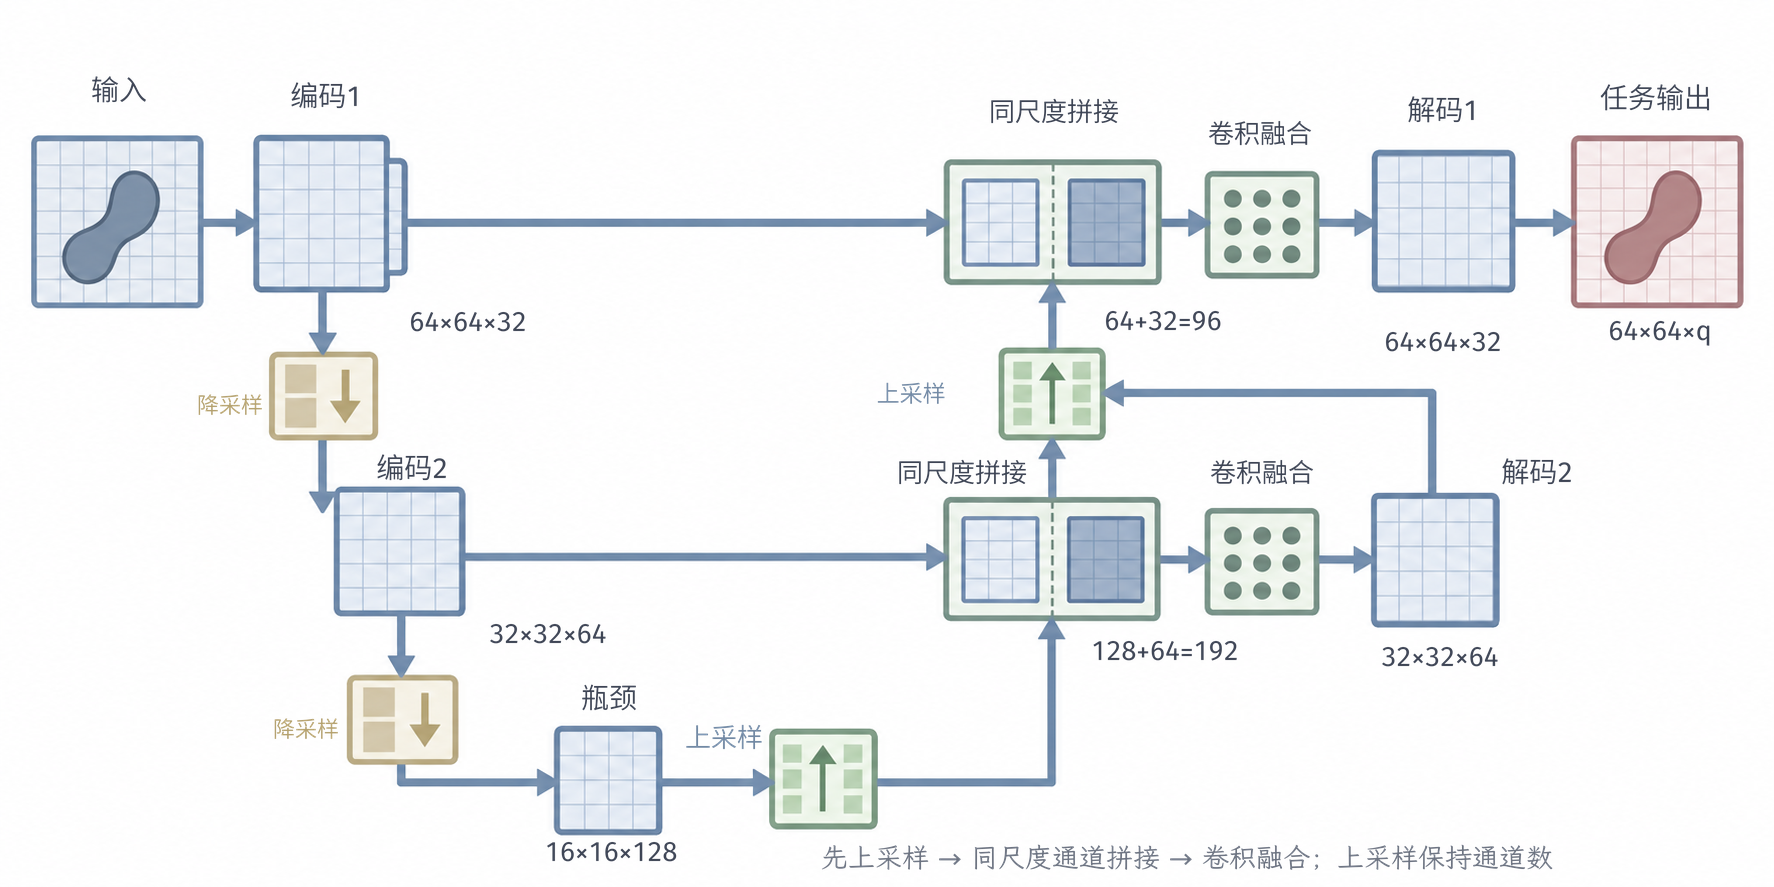
\includegraphics[width=150.199mm]{figures/05-neural-network-models/00-shared/generated/cnn-encoder-decoder/figure.png}
  \caption{用于分割或着色的三尺度编码器—解码器。平面特征片表示特征张量，标签给出空间尺寸和通道数。每级解码先上采样到下一尺度，再在同尺度拼接框中沿通道合并编码特征，随后卷积融合；横向跳跃连接均接入拼接节点。图中上采样保持通道数，因此两次拼接分别得到$128+64=192$和$64+32=96$个通道，卷积后变为64和32个。输出头产生$q$个类别得分或两个颜色通道；采用same卷积，省略原始U-Net的裁剪。}
  \label{fig:cnn-encoder-decoder}
\end{figure*}

跳跃连接为何有助于边界定位，可以从一次池化看出来。两个$2\times2$特征窗口分别只有左上角和右上角为一，其余位置为零；最大池化都输出一，粗网格上已无法据此区分响应原来在哪一侧。仅把这个一插值到更多位置，不能恢复已经舍去的区别。图~\ref{fig:cnn-encoder-decoder}中的横向连接把池化前仍保留位置的编码特征送到解码器，解码卷积便能把这些细节与较深层的上下文共同使用。是否形成正确边界还需要训练监督，连接本身只是提供原先缺少的信息来源。

\term{上采样}（upsampling）是增加网格分辨率的操作。可以先用最近邻或双线性插值生成更密的网格，再用普通卷积处理；也可以用转置卷积共同完成位置扩展与可学习变换。插值方式、目标尺寸和坐标对齐约定都要固定。输入高、宽若不能被总下采样倍数整除，可以在进入网络前填充、在输出后裁剪，或显式按目标尺寸上采样；拼接还要求两个空间轴对齐。

训练时，每张图像提供像素标签，网络按式\eqref{eq:cnn-segmentation-loss}计算损失，再联合更新编码器、解码器和输出头。未标注位置通过掩码排除；若少数类别被大量背景像素淹没，可以在明确权重和归一化后使用加权损失。推理时不需要标签，在各位置取最大得分类别，得到与目标网格对齐的分割图。像素准确率可能主要反映背景，因此评价还需按任务检查区域重叠和边界质量，具体指标在图像处理部分展开。

跨尺度连接把编码器仍保存的细节送给解码器。小目标能否保留，取决于输入分辨率和下采样过程；预测边界的监督又来自标注质量。解码层数、损失和连接方式需要与这些信息来源共同配置。

\FloatBarrier

\subsection{图像生成}
\label{sec:cnn-colorization}

分割的目标是离散类别，另一类空间输出任务则要在每个位置生成连续数值。灰度图着色就是一个直观例子：灰度图只提供亮暗信息，而同样亮度的区域可以对应完全不同的颜色，因此着色是一个\term{条件图像生成}（conditional image generation）问题——给定输入图像，生成一张与它相容的彩色图。本节沿用编码器—解码器，重点说明空间输出如何形成；同时也会暴露一个生成任务特有的困难：当同一个输入存在多种合理答案时，简单地最小化平均误差会得到“四不像”的平均结果。

采用Lab颜色表示时，一个通道描述亮度，另外两个通道描述颜色差异。把亮度按固定规则归一化为输入$\bm X\in\mathbb R^{h\times w\times1}$，将训练彩色图的两个颜色通道按预定尺度变为目标$\bm C\in\mathbb R^{h\times w\times2}$。编码器读取亮度中的边缘、纹理和上下文，解码器恢复颜色的空间分布，最后用$1\times1$卷积输出两个通道。若目标被缩放到$[-1,1]$，可以在输出使用Tanh；采用线性输出时，则需在转换与显示环节处理范围。归一化常数、反归一化和颜色空间转换必须一致，转成RGB后还要处理显示色域。

最直接的教学模型产生确定的颜色估计$\widehat{\bm C}=\bm f_{\bm\theta}(\bm X)$，用像素平方损失训练：
\begin{equation}
  \ell_{\mathrm{col}}=\frac1{hw}\sum_{i=0}^{h-1}\sum_{j=0}^{w-1}
      \lVert\widehat{\bm C}_{i,j,:}-\bm C_{i,j,:}\rVert_2^2\text{。}
  \label{eq:cnn-colorization-loss}
\end{equation}
分割与着色的主体可以采用相同的空间结构，但分割在每个位置输出类别概率，着色在这里输出两个连续值。使用时，将预测颜色反归一化，与输入亮度组合，再转换成彩色图像；模型不应无意中改变输入与输出的空间对齐。

平方损失还有一个与任务有关的限制。在颜色具有有限二阶矩且预测函数可自由选择时，条件平方损失的最优预测是$\mathbb E[\bm C\mid\bm X]$。若同一个灰度输入可能对应多种相距较远的颜色，平均值未必是一种合理着色；例如红与绿的平均可能降低饱和度。Zhang等将颜色空间离散成候选颜色，预测每个位置的颜色分布，用分类目标保留这种多解性，并讨论了平方损失的平均效应\scite{zhang2016colorization}

用一个简化的颜色坐标可以看清这种平均怎样产生。固定灰度输入和一个像素，假设其归一化颜色向量以相同概率取$(1,0)$或$(-1,0)$。确定性预测为$(t,s)$时，条件平均平方损失为$\tfrac12[(t-1)^2+s^2]+\tfrac12[(t+1)^2+s^2]=t^2+s^2+1$，在$(t,s)=(0,0)$处最小。这个最优预测处于两个可能颜色之间，却不是例子中任一种实际颜色。将输出改为候选颜色概率，才有可能分别保留这两种选择，而不是在训练目标中把它们合成一个平均值。

若把输出头改为$q_{\mathrm{col}}$个颜色得分，就可以逐位置归一化为候选颜色概率，再按约定选择、平均或采样得到颜色。各位置分别归一化给出局部候选概率，整张图像的空间协调还依赖它们之间的联合关系。若希望对同一输入生成多个整体协调的结果，还需要引入随机变量并设计相应的分布学习目标。本节的确定性模型把亮度、上下文和颜色估计连接起来；完整的条件生成还要建模同一亮度输入下多种协调颜色之间的分布。

\section{本章小结}
\label{sec:cnn-summary}

本章围绕开篇的问题——如何让网络保留空间结构并在多处复用同一识别规则——展开，可以收为五条主线。

第一，卷积网络用\textbf{局部连接}把每次计算限定在一个邻域内，用\textbf{参数共享}让同一组权重在所有位置复用，直接回应了全连接网络参数爆炸、无法平移复用的困难；多通道则让每个位置并行保存不同的局部特征。非线性激活与逐层组合把局部的边缘、纹理逐级拼成更大范围的判断。

第二，卷积这一运算由若干可独立调节的约定精确定义：数学卷积含核翻转而网络常用省略翻转的互相关；填充处理边界、步幅改变窗口间隔、空洞扩大核内采样间距、转置卷积则把局部贡献反向分配回去（用于上采样而非恢复信息）。明确这些约定，才能一致地计算输出尺寸、实现运算和推导梯度。

第三，计算算法与工程实现是两个层面：直接求和、矩阵化（im2col加GEMM）和Winograd、FFT等变换方法在精确算术下得到相同结果，却有不同的运算量、工作区和数值代价；分块、隐式GEMM、间接卷积和算子融合则进一步改变存储复用与访存。

第四，共享结构决定了梯度的两种累加：同一核权重在各位置的贡献要沿位置累加，一个输入在各重叠窗口的贡献要沿窗口累加；链式法则通过前向映射的转置把输出梯度分配回输入。残差相加、Highway门控和DenseNet拼接则为超深网络提供了不同的信息和梯度近道，以缓解退化问题，同时带来各自的通道规模与内存成本。

第五，结构约束是双刃剑：它在数据符合规则网格、局部相关和平移重复等假设时提升样本效率，但池化和不变性读出一旦删除了任务所需的位置信息，再大的网络也无法恢复；预测的可靠性仍取决于结构是否保留目标信息、样本是否提供足够的独立证据，以及优化能否得到合理解。分割与着色把这些要点综合起来：编码器构造大上下文，解码器恢复空间输出，跳跃连接把下采样前的细节送回去，而输出头和损失决定最终答案表示的是类别、连续值还是不确定性。

\paragraph{扩展阅读}
Goodfellow等教材第9章进一步讨论卷积、共享与池化的结构假设\scite{goodfellow2016}。早期文档识别中的实际配置可结合第~\ref{sec:cnn-lenet}节的LeNet-5与原论文阅读，注意边界、降采样及读出方式怎样配合任务。
